% !TeX root = ../tfg.tex
% !TeX encoding = utf8

\chapter{Análisis Empírico del Deep Double Descent}\label{ch:analisis-empirico-ddd}

En este capítulo abordaremos, de manera práctica, el \textit{Deep Double Descent}. Comenzaremos con su estudio en ejemplos sencillos de regresión, lo cual nos permitirá obtener una primera visión clara e intuitiva de su comportamiento. A continuación y utilizando redes neuronales, se presentarán los principales tipos identificados por la comunidad científica. Asimismo, se explorarán algunos casos adicionales que, si bien no han sido tan estudiados, poseen una relevancia significativa en su análisis.

\section{Materiales y métodos}\label{sec:materiales-y-metodos}

\subsection{\textit{Datasets}}\label{subsec:datasets}

En la parte práctica de este proyecto, se emplearán diversos conjuntos de datos (\textit{datasets}) etiquetados, pues nos movemos bajo el enfoque del aprendizaje supervisado. Dado que la experimentación se limita a este tipo de aprendizaje, se han seleccionado \textit{datasets} ampliamente reconocidos y utilizados en problemas de clasificación de imágenes, lo que también nos ayudará a comparar los resultados obtenidos con los de la comunidad científica. A continuación, se detallarán los principales \textit{datasets} utilizados en este estudio: MNIST, CIFAR$10$ y CIFAR$100$.

Cabe destacar que, aunque en este proyecto también se utilizan \textit{datasets} sintéticos, estos no serán mencionados en esta sección, pues se detallarán en el propio experimento, y la descripción se centrará exclusivamente en los conjuntos de datos comentados anteriormente.

\subsubsection{MNIST}\label{subsubsec:MNIST}

El dataset MNIST (Modified National Institute of Standards and Technology)~\cite{LeCun1998} es un conjunto de datos de imágenes ampliamente utilizado para tareas de clasificación. Consta de $70000$ imágenes en escala de grises de dígitos escritos a mano, las cuales se dividen en $60000$ imágenes para entrenamiento y $10000$ para test. Además, cada imagen tiene un tamaño de $28 \times 28$ píxeles.

\subsubsection{CIFAR10 y CIFAR100}\label{subsubsec:CIFAR10-y-CIFAR100}

CIFAR$10$~\cite{Krizhevsky2009} es un conjunto de datos utilizado para tareas de clasificación. Consta de $60000$ imágenes en color, distribuidas en $10$ clases diferentes, cada una con $6000$ imágenes. A su vez, estas imágenes se dividen en $50000$ imágenes para entrenamiento y $10000$ para test. Cada imagen tiene un tamaño de $32 \times 32$ píxeles y está en formato RGB, es decir, cuenta con $3$ capas, cada una asociada con un color del formato RGB.

Por otro lado, CIFAR$100$~\cite{Krizhevsky2009} es un conjunto de datos similar a CIFAR$10$, pero con $100$ clases. Consta de $60000$ imágenes en color, divididas en $100$ clases de $600$ imágenes cada una, con $500$ para entrenamiento y $100$ para test. Las imágenes tienen un tamaño de $32 \times 32$ píxeles en formato RGB.

Para terminar esta sección, se presenta una tabla a modo de resumen de los \textit{datasets} que se utilizarán en este proyecto. La Tabla~\ref{tab:datasets} muestra la información relevante sobre cada uno, incluyendo el número total de imágenes, el tamaño de las imágenes y el número de características (píxeles totales), lo que proporciona una visión general de sus características principales y facilita la comparación entre ellos.

\begin{table}[h]
    \centering
    \begin{tabular}{|c|c|c|c|c|}
    \hline
    \textbf{Dataset} & \textbf{Nº imágenes} & \textbf{Tamaño imagen} & \textbf{Clases} & \textbf{Entrada} \\
    \hline
    MNIST & $70000$ & $28 \times 28$ píxeles (escala de grises) & $10$ & $784$ \\
    CIFAR$10$ & $60000$ & $32 \times 32$ píxeles (RGB) & $10$ & $3072$ \\
    CIFAR$100$ & $60000$ & $32 \times 32$ píxeles (RGB) & $100$ & $3072$ \\
    \hline
    \end{tabular}
    \caption[Resumen de los \textit{datasets} utilizados.]{Resumen de los \textit{datasets} utilizados. En la tabla aparecen sus principales características, donde la última columna hace referencia al número total de píxeles de cada imagen.}\label{tab:datasets}
\end{table}

Aunque los \textit{datasets} elegidos no son excesivamente grandes, con el fin de acelerar el proceso de entrenamiento durante un alto número de épocas, se utilizarán subconjuntos de estos en los experimentos. En particular, cuando se haga uso de un subconjunto, se empleará la siguiente notación:

\[
    \textit{dataset}[\text{\textit{train}/\textit{test}}]
\]

donde \textit{dataset} se refiere a uno de los conjuntos de datos previamente definidos, \textit{train} indica el número de ejemplos utilizados para entrenamiento, y \textit{test} representa el número de ejemplos en el conjunto de test. Un ejemplo sería MNIST[$4000/1000$], donde se indica que estamos utilizando un subconjunto de MNIST con $4000$ ejemplos de entrenamiento y $1000$ para test.

\subsection{Protocolo de validación experimental}\label{subsec:protocolo-experimental}

Para la validación y estimación del rendimiento de cada modelo, se emplea la técnica conocida como \textit{hold-out}. Esta técnica consiste en dividir el conjunto de datos en dos subconjuntos: uno destinado al entrenamiento del modelo y otro para la evaluación de su rendimiento (véase la imagen izquierda de la Figura~\ref{fig:protocolos}). En este enfoque, el conjunto de entrenamiento se utiliza para ajustar el modelo, mientras que el conjunto de test se emplea para evaluar su capacidad de generalización frente a datos no vistos previamente. 

\begin{figure}[h]
    \centering
    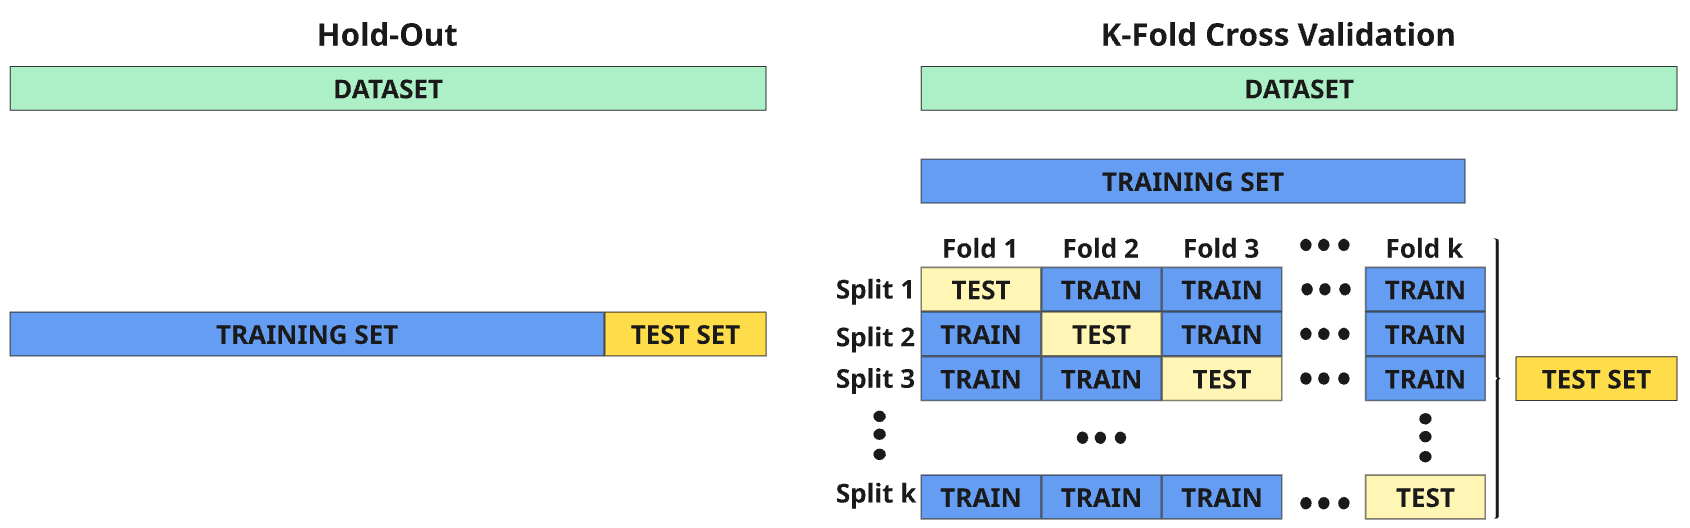
\includegraphics[width=0.8\linewidth]{img/protocolo-experimental.png}
    \caption[Protocolos de validación experimental.]{Protocolos de validación experimental. A la izquierda se muestra la técnica \textit{hold-out}, en la que el conjunto de datos se divide en dos subconjuntos: uno para el entrenamiento y otro para test. A la derecha se presenta \textit{$K$-fold cross validation}, donde el conjunto de entrenamiento se divide en $K$ pliegues, siendo uno de ellos utilizado como conjunto de test.}\label{fig:protocolos}
\end{figure}

Es importante destacar que el método habitualmente preferido para la validación de modelos suele ser la validación cruzada o \textit{$K$-fold cross validation}. Esta técnica consiste en dividir el conjunto de entrenamiento en $K$ subconjuntos o pliegues (véase la imagen derecha de la Figura~\ref{fig:protocolos}), donde en cada iteración uno de estos subconjuntos se utiliza como conjunto de test, mientras que los demás se emplean como conjunto de entrenamiento. Este proceso se repite hasta que cada subconjunto haya sido utilizado como conjunto de test en al menos una iteración. Así, cuando se utiliza un valor de $K = 1$, esta técnica se reduce a un \textit{hold-out}, lo que permite considerarla como una extensión de la misma. De este modo, se obtiene una estimación más robusta del rendimiento del modelo frente a datos no vistos previamente. Finalmente, el rendimiento del modelo se evalúa en el conjunto de prueba final, que no ha sido utilizado durante ninguna de las particiones de entrenamiento.

Por tanto, la elección del método \textit{hold-out} se debe a su menor requerimiento de potencia computacional y tiempo, lo cual resulta fundamental, dado que nuestros experimentos son especialmente costosos en ambos aspectos (como se puede constatar en las tablas resumen incluidas en la parte experimental). Las particiones utilizadas para generar los conjuntos de entrenamiento y test de los distintos conjuntos de datos son las predeterminadas que vienen con estos y que se han descrito en la sección anterior.

\subsection{Arquitecturas utilizadas}\label{subsec:arquitecturas}

En esta sección se presentan las tres arquitecturas diseñadas y utilizadas con el objetivo de abordar la tarea de clasificación propuesta por los \textit{datasets} comentados en la sección anterior. Las arquitecturas seleccionadas varían en términos de su complejidad (número de parámetros) y del tipo de capas que incorporan, desde modelos simples hasta configuraciones más profundas. Este enfoque permitirá analizar el impacto del \textit{Deep Double Descent} en los distintos casos que puede presentarse y sobre las distintas arquitecturas. A continuación, se describen en detalle las arquitecturas implementadas, justificando su elección y su relevancia en el contexto de este estudio.

\subsubsection{2NN}\label{subsubsec:2NN}

Como primer modelo se propone una arquitectura muy simple, formada únicamente por dos capas densas (un perceptrón multicapa (MLP) formado por dos capas). Para ello, primeramente se añade una capa de aplanamiento \textit{(flattening)} con el objetivo de convertir las imágenes proporcionadas en la entrada en un vector de píxeles unidimensional. A continuación, se añade la primera capa densa, cuya entrada está compuesta por el vector unidimensional anterior y su salida será un número variable de neuronas, todas ellas conectadas con cada entrada del vector. Finalmente, la última capa densa conectará las neuronas de salida de la primera capa densa con un número de neuronas que será igual al número de clases del datasets con el que estemos trabajando (véase Figura~\ref{fig:arquitecura2nn}).

\begin{figure}[h]
    \centering
    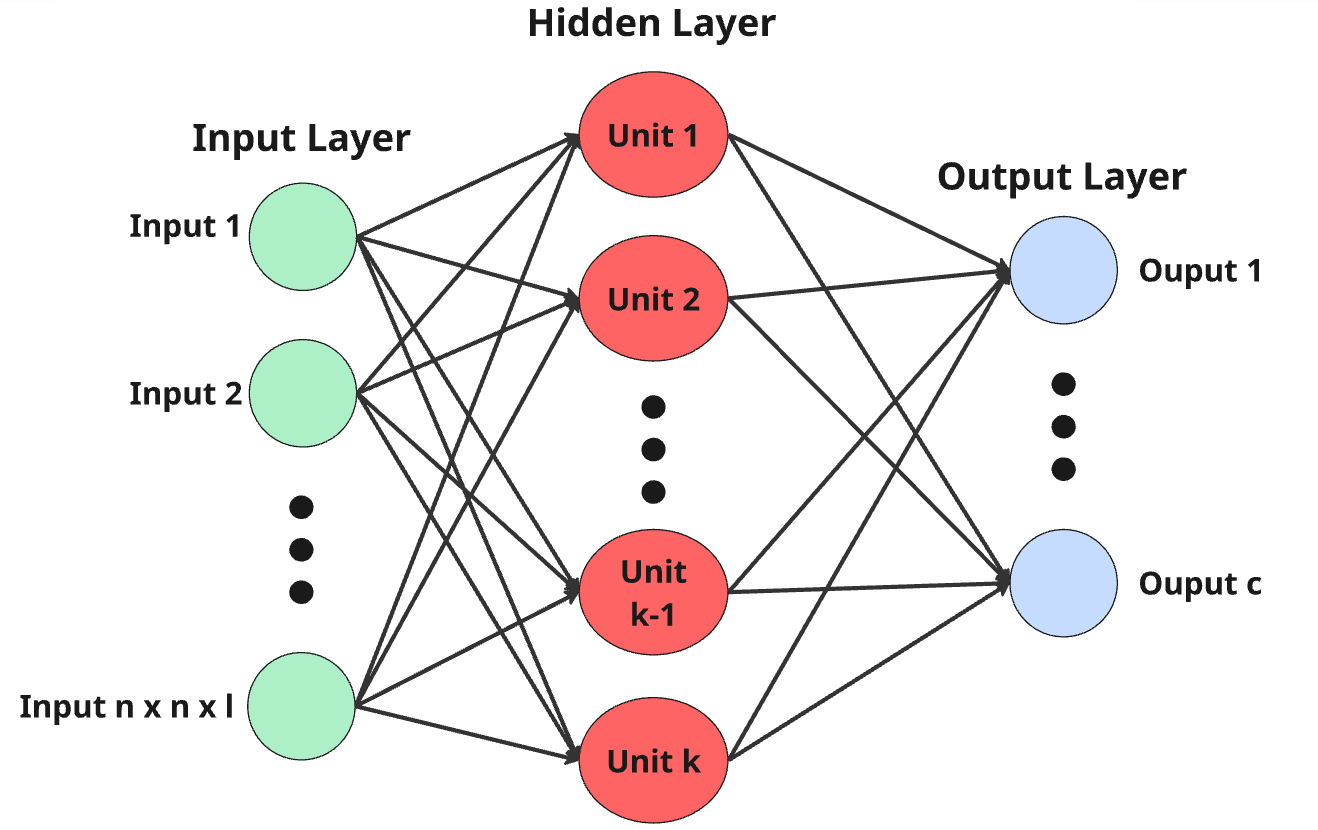
\includegraphics[width=0.6\linewidth]{img/arquitectura2nn.png}
    \caption[Arquitectura $2$NN.]{Arquitectura $2$NN. La capa de entrada está formada por un número de neuronas igual al número de píxeles de la imagen de entrada. Estas neuronas estarán conectadas a todas las neuronas de la capa oculta, y a su vez, estas últimas estarán conectadas a todas las neuronas de la capa de salida, la cual corresponde al número de clases del problema.}\label{fig:arquitecura2nn}
\end{figure}

El diseño y elección de este modelo se basa en su relativa sencillez, lo que lo convierte en una opción ideal para llevar a cabo una amplia variedad de experimentos, ya que tiempos de entrenamiento significativamente más bajos en comparación con otras arquitecturas utilizadas, permitiéndonos estudiar el DDD sin un alto coste computacional. No obstante, dado que los MLPs no cuentan con el \textit{inductive bias} adecuado para trabajar con imágenes, se espera obtener peores resultados en comparación con el uso de CNNs.

Finalmente, se expone una tabla con el número de parámetros que conforman esta arquitectura. Este detalle es especialmente relevante para los experimentos, ya que el número de parámetros reflejará el nivel de complejidad de la arquitectura (véase Tabla~\ref{tab:numero-parametros}).

\begin{table}[ht]
    \centering
    \renewcommand{\arraystretch}{1.5} 
    \begin{tabular}{|c|c|c|c|}
    \hline
    \textbf{Entrada} & \textbf{N° clases} & \textbf{N° unidades} & \textbf{N° parámetros} \\ \hline
    Imagen de tamaño $n \times n \times l$ & c & k & $(n^2 \times l) \times k + k + c \times k + c$ \\ \hline
    \multirow{2}{*}{$28 \times 28 \times 1$} & \multirow{2}{*}{$10$} & $50$ & $39 760$ \\ \cline{3-4}
    & & $100$ & $79 550$ \\ \hline
    \multirow{4}{*}{$32 \times 32 \times 3$} & \multirow{2}{*}{$10$} & $50$ & $118 160$ \\ \cline{3-4}
    & & $100$ & $236 310$ \\ \cline{2-4}
    & \multirow{2}{*}{$100$} & $50$ & $122 750$ \\ \cline{3-4}
    & & $100$ & $245 400$ \\ \hline
    \end{tabular}
    \caption[Resumen de las arquitecturas $2$NN.]{Resumen de las arquitecturas $2$NN. Se muestra el número de parámetros dada una determinada imagen de entrada, donde $k$ hace referencia al número de neuronas de salida de la primera capa densa y $c$ al número de clases del problema de clasificación. Además, se presentan algunos ejemplos de configuraciones.}\label{tab:numero-parametros}
\end{table}

\subsubsection{3CNN}\label{subsubsec:3CNN}

Como segunda arquitectura, se propone una CNN compuesta por $3$ capas convolucionales (denominada $3$CNN), seguidas de capas de \textit{pooling} para reducir dimensionalidad y, finalmente, una capa densa de salida.

Este modelo se presenta como una opción intermedia en términos de complejidad entre el modelo expuesto previamente y el siguiente modelo que se presentará, donde el número de filtros en cada capa se ajustará según un parámetro $k \in \mathbb{N}$, siguiendo la secuencia [$k$, $2k$, $4k$] (véase Figura~\ref{fig:3CNN}).

\begin{figure}[h]
    \centering
    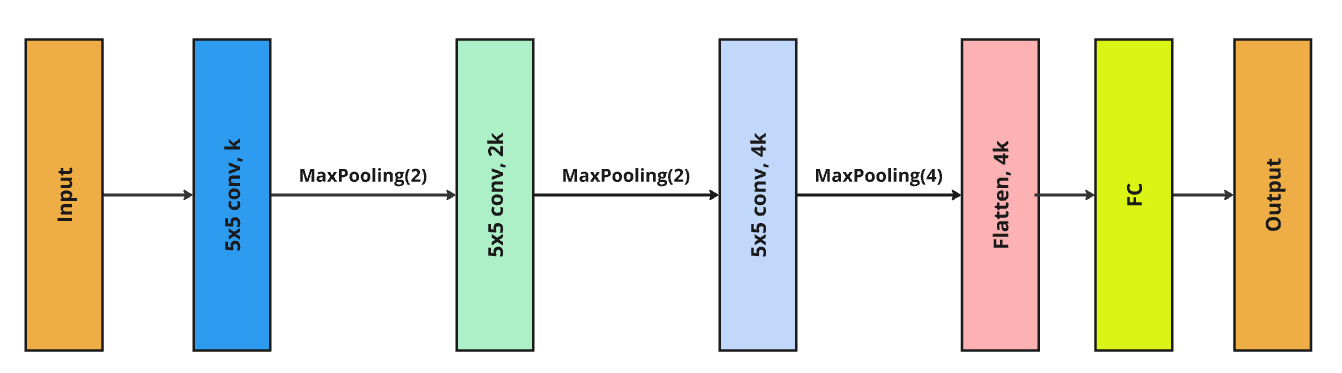
\includegraphics[width=0.8\linewidth]{img/experiments/3CNN.png}
    \caption[Arquitectura $3$CNN.]{Arquitectura $3$CNN. Podemos observar los $3$ bloques convolucionales (distinguidos por color), cada uno de ellos con su correspondiente número de filtros ([$k$, $2k$, $4k$] con $k \in \mathbb{N}$) y las correspondientes capas de \textit{pooling}.}\label{fig:3CNN}
\end{figure}

Finalmente y dado que el número de parámetros asociados a esta arquitectura es tedioso de indicar (debido a la cantidad de capas que la conforman), se exponen en la Tabla~\ref{tab:numero-parametros3cnn} los principales valores del parámetro $k$ (número de filtros) utilizados en el desarrollo del proyecto, lo que permite realizar una comparación con la arquitectura $2$NN anterior y con la siguiente. Cabe destacar que la última capa de \textit{pooling} es adaptativa, lo que permite que la salida tenga dimensiones fijas independientemente del tamaño de la imagen de entrada. No obstante, el número de parámetros experimentará una variación mínima al utilizar imágenes en formato escala de grises o en RGB, puesto que el número de capas permanecerá inalterado.

\begin{table}[ht]
    \centering
    \begin{tabular}{|c|c|c|}
    \hline
    \textbf{Valor de $k$}           & \textbf{Número de parámetros}                     
    \\ \hline
    $20$                  & $\approx 103$\space K                                            \\ \hline
    $45$                  & $\approx 512$\space K                                             \\ \hline
    $64$                  & $\approx 1,03$\space M                                             \\ \hline
    \end{tabular}
    \caption[Número de parámetros de las arquitecturas $3$CNN.]{Número de parámetros de las arquitecturas $3$CNN. Se muestra el número total de parámetros para una entrada de tamaño $32 \times 32 \times 3$, considerando distintos valores del parámetro $k$ y para $10$ clases de salida.}\label{tab:numero-parametros3cnn}
\end{table}

\subsubsection{ResNet18 modificada}\label{subsubsec:resnet18-modificada}

ResNet$18$ es una de las variantes de la famosa arquitectura de redes neuronales convolucionales ResNet (\textit{Residual Networks}), propuesta por Kaiming He y su equipo en $2015$~\cite{He2015}. Esta arquitectura fue diseñada con el objetivo de resolver el problema de la degradación del rendimiento a medida que aumentaba la profundidad de las redes neuronales. ResNet introduce el concepto de conexiones residuales, que permiten que el flujo de información pase a través de capas sin ser afectado por los gradientes de las capas anteriores (véase Apéndice~\ref{ap:apendiceD}).

ResNet$18$, como su nombre indica, tiene $18$ capas de profundidad. Su arquitectura presenta varios bloques de convolución seguidos de conexiones residuales, que permiten que la entrada de cada bloque se sume a la salida de dicho bloque. La primera capa convolucional utiliza un filtro de tamaño $7 \times 7$ y, acto seguido, aparecen los bloques convolucionales formados por $4$ capas convolucionales idénticas, donde cada bloque está formado por dos capas convolucionales con conexiones residuales conectadas con la salida de la segunda capa convolucional. Finalmente, aparece una capa densa que será la salida de la red (véase Figura~\ref{fig:resnet18} para más detalle).

\begin{figure}[h]
    \centering
    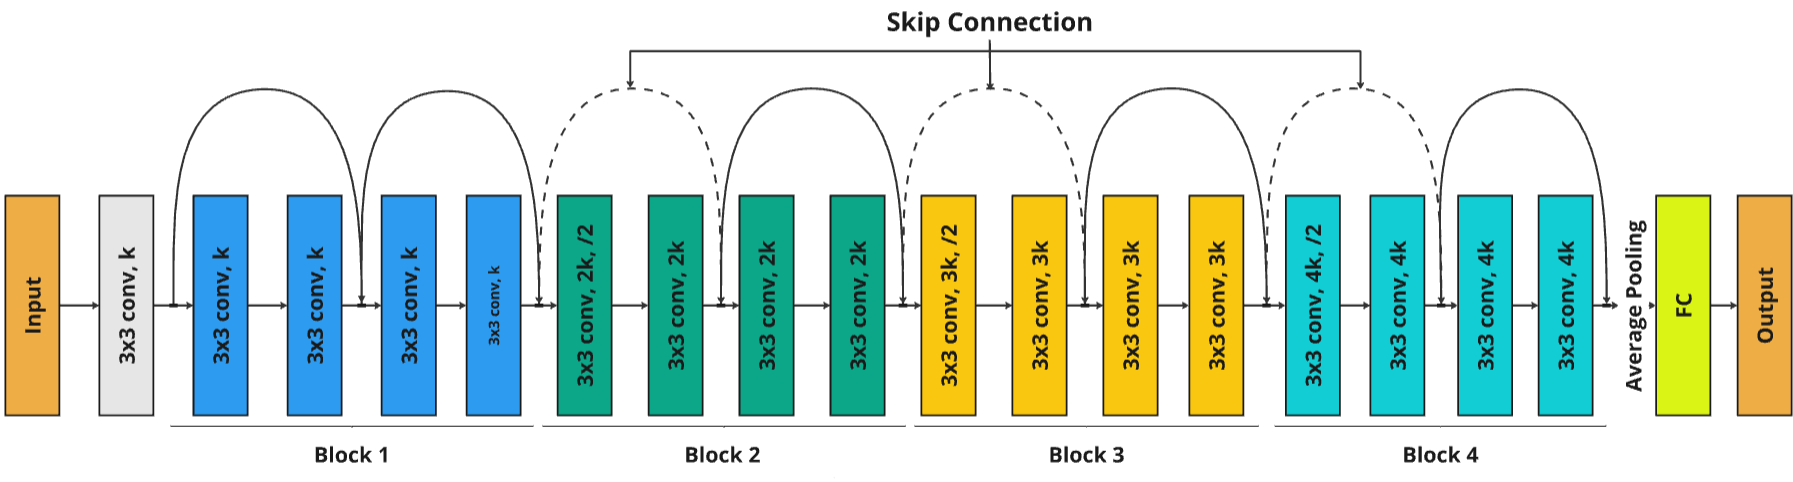
\includegraphics[width=\linewidth]{img/experiments/resnet18modified.png}
    \caption[Arquitectura ResNet$18$ modificada.]{Arquitectura ResNet$18$ modificada. Podemos observar los $4$ bloques convolucionales (distinguidos por color), cada uno de ellos con su correspondiente número de filtros ([$k$, $2k$, $3k$, $4k$] con $k \in \mathbb{N}$), junto con las conexiones residuales.}\label{fig:resnet18}
\end{figure}

La arquitectura que usaremos durante el transcurso de los experimentos (PreActResNet$18$) es una modificación de la arquitectura ResNet$18$ original, dado que en la arquitectura original el número de filtros usados en cada bloque convolucional es [$64$, $128$, $256$, $512$], mientras que en nuestro caso será un número variable $k \in \mathbb{N}$, con el propósito de crear ``distintas'' arquitecturas. Para ello, usaremos como número de filtros para cada bloque convolucional la secuencia: [$k$, $2k$, $3k$, $4k$]~\cite{Nakkiran2019}, con el objetivo de comparar los resultados obtenidos con los de la literatura existente. Destacamos que, para el valor $k=64$, nuestra arquitectura es la propia arquitectura ResNet$18$ original. Además, de manera similar a la arquitectura anterior, se utiliza \textit{pooling} adaptativo en la última capa para preservar un tamaño de entrada común a la capa densa, independientemente del tamaño de entrada a la red.

Finalmente, y al igual que en la arquitectura anterior, se presenta una tabla con los principales valores del parámetro $k$ utilizados en el desarrollo del proyecto (véase Tabla~\ref{tab:numero-parametrosresnet}), con el propósito de permitir una comparación directa de ambas arquitecturas.

\begin{table}[ht]
    \centering
    \begin{tabular}{|c|c|c|}
    \hline
    \textbf{Valor de $k$}           & \textbf{Número de parámetros}                     
    \\ \hline
    $20$                  & $\approx 1.1$\space M                                            \\ \hline
    $45$                  & $\approx 5.5$\space M                                             \\ \hline
    $64$                  & $\approx 11.1$\space M                                             \\ \hline
    \end{tabular}
    \caption[Número de parámetros de las arquitecturas ResNet$18$ modificadas.]{Número de parámetros de las arquitecturas ResNet$18$ modificadas. Se muestra el número de parámetros dado un determinado valor $k$ y para $10$ clases de salida.}\label{tab:numero-parametrosresnet}
\end{table}

\subsection{Hiperparámetros}\label{subsec:hiperparametros}

Los hiperparámetros que serán utilizados a lo largo de la experimentación, por lo general, son los valores por defecto que vienen con las implementaciones estándar de Pytorch~\cite{NEURIPS2019_9015} de los distintos métodos utilizados. Las únicas modificaciones que se han realizado son aquellas necesarias para replicar experimentos descritos en la literatura existente y, en dichos casos, se indicarán específicamente en el propio experimento.

En cuanto al tamaño de lote (\textit{batch size}), variará entre $128$ y $256$, siendo este último el valor por defecto, de manera similar a la literatura existente, lo que representa un valor relativamente alto, con el objetivo de acelerar el entrenamiento. Respecto a la tasa de aprendizaje del optimizador utilizado (Adam en nuestro caso\footnote{No obstante, aunque se utilice Adam como optimizador debido a su versatilidad, resultados similares se obtienen para SGD, como se puede observar en~\cite{Nakkiran2019}.}), se empleará su tasa por defecto. El uso de distintos valores para \textit{batch size} y \textit{learning rate} en un problema donde se manifiesta el doble descenso se pueden observar en el Apéndice~\ref{ap:apendiceB}, donde se muestra que, si el fenómeno ocurre, el tamaño del lote utilizado y la tasa de aprendizaje no afectan significativamente al comportamiento del mismo. Finalmente, el número de épocas por defecto son $1000$.

Por otra parte, cabe destacar que, salvo que se indique lo contrario, no se introduce ninguna técnica de regularización en los experimentos realizados, debido a que el \textit{Deep Double Descent} se observará sin la influencia de las mismas. De este modo, se pretende estudiar cómo se manifiesta este suceso bajo condiciones más puras, sin modificaciones que podrían alterar sus efectos. Cualquier variación en este aspecto será especificada de manera explícita en el propio experimento. Adicionalmente, como función de pérdida a minimizar se utilizará la entropía cruzada, dado que estamos trabajando con problemas de clasificación multiclase.

\section{Experimentos}\label{sec:experimentos}

En esta sección se presentará una batería de resultados obtenidos a partir de los experimentos realizados, los cuales incluyen tanto resultados favorables como desfavorables, con el propósito de proporcionar una visión lo más completa posible de los mismos. La Tabla~\ref{tabla:resumen-experimentos-intro} sirve como introducción a los distintos experimentos que se desarrollarán en esta sección.

Todo el código desarrollado, así como los distintos resultados obtenidos, pueden encontrarse en el GitHub \url{https://github.com/jantonioruiz/Deep-Double-Descent}. De esta manera, se combinan Git y GitHub con el propósito de llevar un control de versiones.

\begin{table}[h]
    \centering
    \small 
    \renewcommand{\arraystretch}{0.9} 
    \begin{NiceTabular}{c c c}[hvlines,color-inside]
        \Block[fill={cyan!50}]{2-1}{\textbf{Experimento}} & \Block[fill={cyan!50}]{2-1}{\textbf{Descripción}} & \Block[fill={cyan!50}]{2-1}{\textbf{Subsección}} \\ \\
        
        \Block{5-1}{Aproximación \\ polinómica} & \Block{5-1}{Comenzamos empleando aproximación polinómica, con el objetivo \\ de disponer de resultados preliminares que nos permitan concluir \\ si somos capaces de reproducir la aparición del doble descenso.} & \Block{5-1}{\ref{subsec:approx-polinomica}} \\ \\ \\ \\ \\

        \Block{5-1}{\textit{Noise-wise} \\ \textit{double-descent}} & \Block{5-1}{Analizaremos el impacto del ruido tanto en su aparición \\ como en la localización del umbral de interpolación.} & \Block{5-1}{\ref{subsec:noise-wise-dd}} \\ \\ \\ \\ \\

        \Block{5-1}{\textit{Sample-wise} \\ \textit{double-descent}} & \Block{5-1}{Estudiaremos el impacto del número de ejemplos en la localización \\ del umbral de interpolación, tratando de mostrar cómo existe una \\ región en la que entrenar con más ejemplos empeora el rendimiento.} & \Block{5-1}{\ref{subsec:sample-wise-dd}} \\ \\ \\ \\ \\

        \Block{5-1}{\textit{Model \& Epoch-wise} \\ \textit{double-descent}} & \Block{5-1}{Exploraremos en profundidad el doble descenso \\ asociado a la complejidad del modelo y al número de épocas, \\ utilizando los diversos conjuntos de datos y arquitecturas.} & \Block{5-1}{\ref{subsec:model-epoch-wise}} \\ \\ \\ \\ \\

        \Block{5-1}{\textit{Width vs Depth} \\ \textit{double-descent}} & \Block{5-1}{Investigaremos el fenómeno al usar redes de mayor profundidad \\ en lugar de mayor anchura, con el propósito de evaluar su \\ robustez frente a la arquitectura empleada.} & \Block{5-1}{\ref{subsec:width-depth}} \\ \\ \\ \\ \\

    \end{NiceTabular}
    \caption{Resumen de las ideas principales de los experimentos realizados.}\label{tabla:resumen-experimentos-intro}
\end{table}

\subsection{Entornos de desarrollo y ejecución}\label{subsec:entornos-desarrollo-ejecucion}

Como preámbulo a los distintos experimentos que se detallan a continuación, se presentan las herramientas utilizadas para su realización. El lenguaje de programación empleado es \textit{Python}, en su versión más reciente ($3.13.3$), debido a su gran facilidad y versatilidad para trabajar con modelos de aprendizaje profundo. Asimismo, se hace uso de las bibliotecas \textit{PyTorch} junto con las necesarias de \textit{CUDA} para el entrenamiento de las diferentes arquitecturas, así como \textit{NumPy} y \textit{Pandas} para el procesamiento de datos, y \textit{Matplotlib} y \textit{Seaborn} para la generación de gráficos.

Por otro lado, se proporcionan \textit{notebooks} de \textit{Google Colab} con el código asociado a los experimentos que no requieren el uso de redes neuronales y que no demandan grandes recursos. Para los experimentos que requieren el uso de redes neuronales (y que son tan costosos que no se pueden realizar en \textit{notebooks}), se proporciona el código en formato \textit{Python} junto con un script de ayuda para lanzar cualquier experimento realizado. Además, para este caso, se incluye en otro cuaderno el código necesario para visualizar las gráficas correspondientes a los resultados obtenidos por los modelos neuronales, con el propósito de evitar tener que ejecutar ningún proceso adicional para su visualización.

El proceso de ejecución de los experimentos que utilizan redes neuronales se lleva a cabo en los nodos de cómputo (GPUs) de los servidores de la Universidad de Granada (UGR), a los cuales se accede de forma remota mediante SSH. Para el envío de los experimentos, se emplea un \textit{script} de Shell en el que se especifican tanto los parámetros del experimento como el nodo a utilizar. El servidor hace uso de SLURM como gestor de colas, siendo este el encargado de reservar los recursos necesarios en la partición ``dios'' del servidor. Finalmente, se utiliza la herramienta \textit{Conda} para gestionar tanto los entornos como los paquetes, asegurando que se disponga de todas las bibliotecas necesarias.

Dado que nuestra experimentación es excesivamente costosa, hacemos uso de tres nodos de cómputo, de manera indistinta, dentro de la partición ``dios'' de los servidores. Las especificaciones de estos nodos se detallan a continuación:

\begin{enumerate}
    \item Nodo \textbf{atenea}: Cuenta con dos procesadores Intel Xeon E5-$2630$, $128$GB de memoria RAM DDR$4$ y cuatro tarjetas gráficas GTX Titan Xp.
    \item Nodo \textbf{hera}: Cuenta con dos procesadores Intel Xeon $4114$, $128$GB de memoria RAM DDR$4$ y cuatro tarjetas gráficas Titan RTX.
    \item Nodo \textbf{dionisio}: Cuenta con dos procesadores Intel Xeon Silver $4216$, $512$GB de memoria RAM DDR$4$ y dos tarjetas gráficas Quadro RTX $8000$.
\end{enumerate}

Aunque estos nodos cuentan con especificaciones diferentes, ofrecen resultados similares en cuanto a tiempo de ejecución. Este hecho permite que puedan ser utilizados de manera paralela para acelerar los cálculos, ofreciendo tiempos de ejecución significativos para la comparación de resultados.

Finalmente, cabe destacar que, a principios del mes de abril, se comunicó que el uso de las GPUs de la Universidad de Granada quedaba limitado a un máximo de $12$ horas de ejecución continuada. Esta limitación a nivel de hardware complica la realización de algunos experimentos, dado que, en este proyecto, es necesario llevar el entrenamiento de los modelos mucho más allá de este tiempo. De este modo, los experimentos realizados tras esta comunicación presentan configuraciones de parámetros distintas en comparación con el resto. Es importante resaltar que la batería experimental llevada a cabo en este proyecto es de gran calibre, lo que conlleva una mayor demanda de recursos y tiempo de ejecución para obtener resultados más precisos y concluyentes.

\subsection{Aproximación polinómica}\label{subsec:approx-polinomica}

Este experimento sirve como preámbulo al resto de experimentos y tiene como objetivo proporcionar una comprensión clara y sencilla de por qué puede manifestarse el \textit{Deep Double Descent} al aumentar la complejidad de un modelo. A través de este análisis preliminar, se busca sentar las bases para explorar más a fondo cómo la complejidad afecta al comportamiento y rendimiento de los modelos.

Para ello, intentaremos aproximar una función objetivo mediante tres enfoques distintos: el primero basado en la base de Legendre, el segundo empleando la base polinómica clásica, y el tercero utilizando una base polinómica redundante, donde en todos los casos usaremos un número finito de puntos muestreados de dicha función objetivo para realizar esa aproximación. Este experimento no empleará redes neuronales, sino que se basará en una simple regresión polinómica, cuya solución obtendremos mediante la pseudoinversa.

Por tanto, el objetivo de este experimento es encontrar la función $f$ que modele el valor esperado de una variable aleatoria dependiente $y$ (salida) en términos del valor esperado de una variable aleatoria independiente $x$ (entrada), es decir, $f(x)=y$. Dado que la función objetivo es desconocida, buscamos aproximarla, en este caso, mediante el uso de funciones polinómicas. De esta manera, buscamos aproximar la variable $y$ haciendo uso de las siguientes tres aproximaciones:

\begin{table}[h]
    \centering
    \begin{NiceTabular}{c c}[hvlines,color-inside]
        \Block{1-1}{\textbf{Base}} & \Block{1-1}{\textbf{Aproximación}} \\ 
        
        \Block{2-1}{Legendre} & \Block{2-1}{$w_0 \cdot P_0(x) + w_1 \cdot P_1(x) + w_2 \cdot P_2(x) + \cdots + w_n \cdot P_n(x) = y$} \\ \\

        \Block{2-1}{Clásica} & \Block{2-1}{$w_0 \cdot 1 + w_1 \cdot x + w_2 \cdot x^2 + \cdots + w_n \cdot x^n = y$}  \\ \\

        \Block{2-1}{Redundante} & \Block{2-1}{$w_0 \cdot 1 + w_1 \cdot (1 + x) + w_2 \cdot (1 + x + x^2) + \cdots + w_n \cdot (1 + x + \cdots + x^n) = y$}  \\ \\

    \end{NiceTabular}
    \caption{Aproximaciones polinómicas de grado $n$ utilizadas para regresión polinomial.}\label{tabla:aproximaciones-polinomicas}
\end{table}

donde $w = [w_0, w_1, \ldots, w_n]$ representa el vector de parámetros que el modelo aprende durante la fase de entrenamiento y $P_i(x)$ hace referencia al $i$-ésimo polinomio de Legendre\footnote{Los polinomios de Legendre forman un sistema de polinomios completos y ortogonales en el intervalo $[-1, 1]$.}.


Sabemos que la solución de norma mínima para el problema de mínimos cuadrados asociado $Xw=y$ viene dada por la pseudoinversa (véase Sección~\ref{sec:svd-pseudoinversa}), donde, dependiendo de la base elegida, la matriz $X$ viene dada por:

\[
\begin{aligned}
    X_{Legendre} &= 
    \begin{bmatrix}
        P_0(x_0) & P_1(x_0) & \cdots & P_n(x_0) \\
        P_0(x_1) & P_1(x_1) & \cdots & P_n(x_1) \\
        P_0(x_2) & P_1(x_2) & \cdots & P_n(x_2) \\
        \vdots & \vdots & \ddots & \vdots \\
        P_0(x_m) & P_1(x_m) & \cdots & P_n(x_m)
    \end{bmatrix},
    \quad
    X_{Vandermonde} = 
    \begin{bmatrix}
        1 & x_0 & x_0^2 & \cdots & x_0^n \\
        1 & x_1 & x_1^2 & \cdots & x_1^n \\
        1 & x_2 & x_2^2 & \cdots & x_2^n \\
        \vdots & \vdots & \vdots & \ddots & \vdots \\
        1 & x_m & x_m^2 & \cdots & x_m^n
    \end{bmatrix},
\end{aligned}
\]
\vspace{0.5cm}
\[
X_{Redundant} = 
\begin{bmatrix}
    1 & x_0 & 1+x_0^2 & \cdots & 1+x_0+\cdots+x_0^n \\
    1 & x_1 & 1+x_1^2 & \cdots & 1+x_1+\cdots+x_1^n \\
    1 & x_2 & 1+x_2^2 & \cdots & 1+x_2+\cdots+x_2^n \\
    \vdots & \vdots  & \vdots & \ddots & \vdots \\
    1 & x_m & 1+x_m^2 & \cdots & 1+x_m+\cdots+x_m^n
\end{bmatrix},
\]

donde $X_{Legendre}$, $X_{Vandermonde}$ y $X_{Redundant}$ son las matrices $X$ relativas, respectivamente, a la base de polinomios de Legendre, a la base polinómica clásica y a la base polinómica redundante. Así, el vector de parámetros viene dado por $w = X^{\dagger} y$, donde $X^{\dagger}$ es la pseudoinversa de la matriz $X$ asociada a cada aproximación.

\subsubsection{Función lineal}\label{subsubsec:funcion-lineal}

En primera instancia, buscamos aproximar la función objetivo dada por $f(x) = 2x + \cos(25x)$ utilizando $10$ puntos muestreados de esa función y usando la pseudoinversa, con el objetivo de replicar y dar más contexto al experimento presentado en~\cite{Schaeffer2023}. La tendencia de la función objetivo la marca la función lineal $2x$ y la función trigonométrica $\cos(25x)$ nos ayudará a introducir cierto ruido a esa función de tendencia, asimilando el posible ruido que encontramos en el mundo real.

\begin{figure}[h]
    \centering
    \begin{subfigure}[b]{0.48\textwidth}
        \centering
        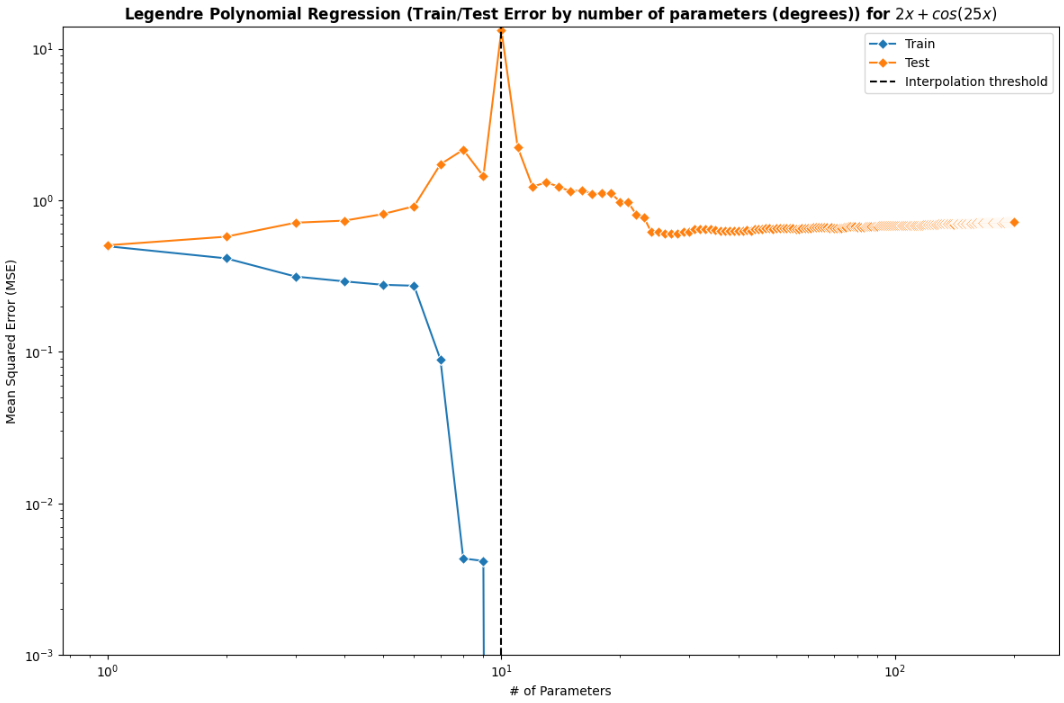
\includegraphics[width=\textwidth]{img/experiments/legendre1DDD.png}
        \caption{Doble descenso para la aproximación polinómica de Legendre.}\label{fig:legendre1.1DDD}
    \end{subfigure}
    \hfill
    \begin{subfigure}[b]{0.48\textwidth}
        \centering
        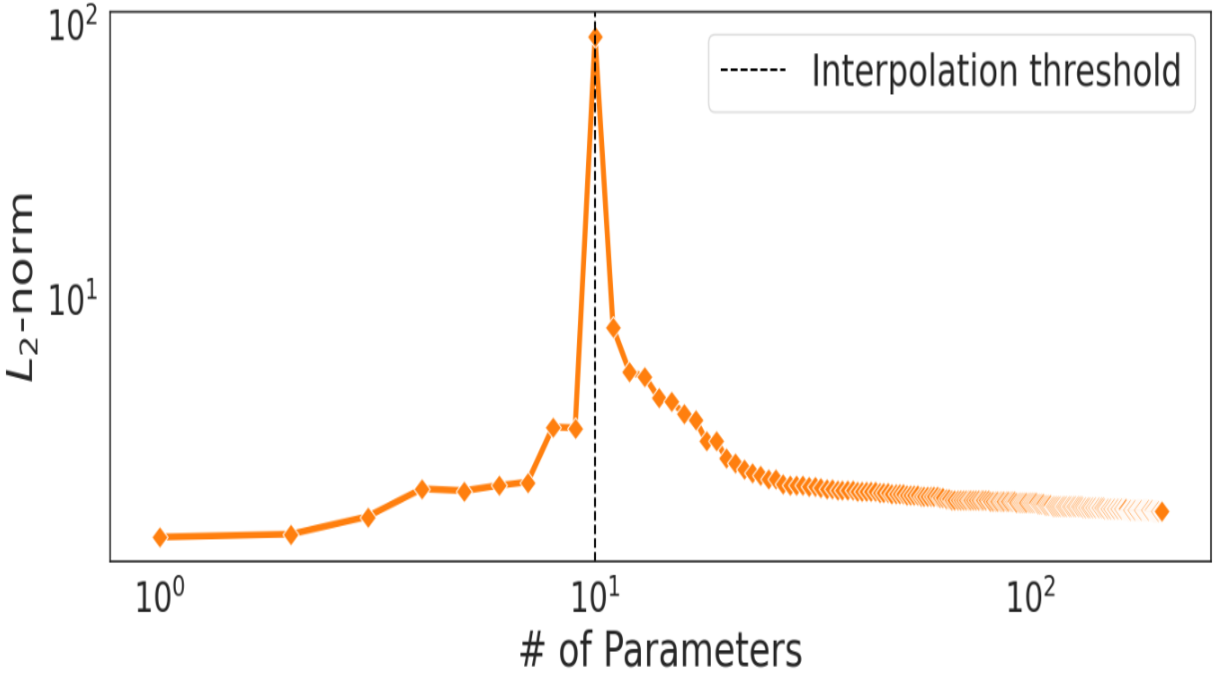
\includegraphics[width=\textwidth]{img/experiments/legendre1.4.png}
        \caption{Norma euclídea del vector de parámetros asociado a cada aproximación.}\label{fig:legendre1.2DDD}
    \end{subfigure}
    \caption[Doble descenso al utilizar aproximación polinómica de Legendre y norma del vector de parámetros.]{Doble descenso al utilizar aproximación polinómica de Legendre, donde el umbral de interpolación corresponde al número de datos de entrenamiento (línea negra punteada), junto con la norma del vector de parámetros asociado, la cual decrece tras dicho umbral.}\label{fig:legendre1DDD}
\end{figure}

Para el caso de la aproximación de Legendre, podemos observar en la Figura~\ref{fig:legendre1.1DDD} cómo se manifiesta el doble descenso. De esta manera, al superar el umbral de interpolación, encontrado justo al usar el mismo número de parámetros que datos de entrenamiento, el error en el conjunto de test vuelve a disminuir, produciéndose el segundo descenso.

Por otro lado, podemos observar en la Figura~\ref{fig:legendre1DD} las distintas aproximaciones que obtiene el modelo al utilizar distinto número de parámetros. Antes de llegar al umbral de interpolación, el modelo no tiene la suficiente capacidad como para ajustarse a cada uno de los datos. Al alcanzar el umbral de interpolación, el modelo se ve obligado a ajustarse exactamente a cada uno de los puntos de entrenamiento, lo que lo convierte en una aproximación única. En este caso, esta ``rigidez'' del modelo no asegura una buena generalización debido a presentar numerosas oscilaciones. Al superar dicho umbral, el aumento en el número de parámetros permite la existencia de múltiples modelos de interpolación para cada grado, facilitando la selección de una opción que generalice bien. De este modo, el modelo adquiere mayor flexibilidad para aproximar los datos, lo que da lugar a una función cada vez más ``suave''.

\begin{figure}[h]
    \centering
    \begin{minipage}{0.32\textwidth}
        \centering
        \textbf{Región infraparametrizada} \\[0.5ex] 
        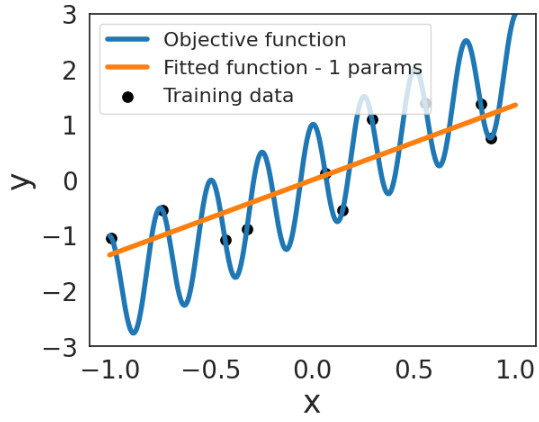
\includegraphics[width=\linewidth]{img/experiments/legendre1.1.png}
    \end{minipage}
    \begin{minipage}{0.32\textwidth}
        \centering
        \textbf{Umbral de interpolación} \\[0.5ex] 
        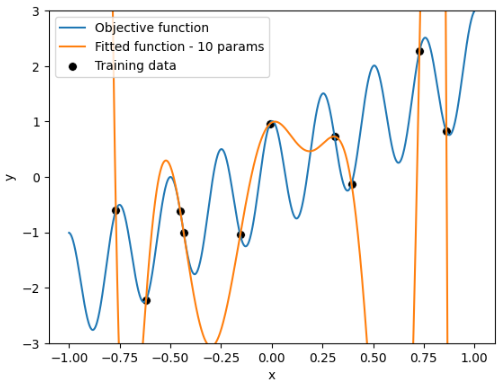
\includegraphics[width=\linewidth]{img/experiments/legendre1.2.png}
    \end{minipage}
    \begin{minipage}{0.32\textwidth}
        \centering
        \textbf{Región sobreparametrizada} \\[0.5ex] 
        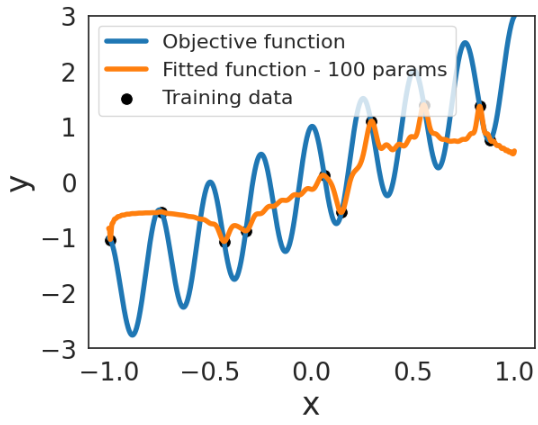
\includegraphics[width=\linewidth]{img/experiments/legendre1.3.png}
    \end{minipage}
    \caption[Intuición del \textit{Deep Double Descent} usando regresión polinómica.]{Intuición del \textit{Deep Double Descent} usando regresión polinómica. Cuando nos encontramos en la región infraparametrizada, el modelo no es capaz de capturar todos los datos de entrenamiento, haciendo que el \textit{bias} del modelo sea grande, aunque la varianza sea pequeña. En el umbral de interpolación, el modelo captura perfectamente todos los datos, haciendo que el \textit{bias} sea pequeño pero la varianza sea grande, pues la función aprendida dependerá de la posición de los datos de entrenamiento. Finalmente, en la región sobreparametrizada, el modelo está regularizado hacia una solución de norma pequeña similar a la inicial.}\label{fig:legendre1DD}
\end{figure}

En la Figura~\ref{fig:legendre1.2DDD} se observa cómo el modelo, a medida que aumenta su capacidad, sigue reduciendo la norma del vector de parámetros aprendido, ligado a que, como se explicó en la Sección~\ref{sec:svd-pseudoinversa}, la pseudoinversa proporciona la solución de norma mínima. No obstante, este comportamiento nos indica que el modelo se va ``autoregularizando'' hacia soluciones cada vez más simples (suaves) y que se asemejan más a la solución inicial (véanse la primera y última imágenes de la Figura~\ref{fig:legendre1DD}), lo cual es coherente con lo expuesto en la parte teórica.

Por otro lado, en las aproximaciones polinómicas clásicas, es posible percibir en la Figura~\ref{fig:aproximaciones-polinomicas} que dicho fenómeno no se presenta, al menos con el mismo número de parámetros, incluso habiendo obtenido un error de entrenamiento nulo. Es por esto que las aproximaciones obtenidas por el modelo a partir del umbral de interpolación son peores (véase Figura~\ref{fig:polynomial1DD}). No obstante, una vez superado el umbral de interpolación, estas aproximaciones clásicas, al igual que la aproximación de Legendre, ofrecen soluciones con menor norma del vector de parámetros, como puede notarse en la Figura~\ref{fig:normas-clasicas}.

\begin{figure}[h]
    \centering
    \begin{subfigure}[b]{0.48\textwidth}
        \centering
        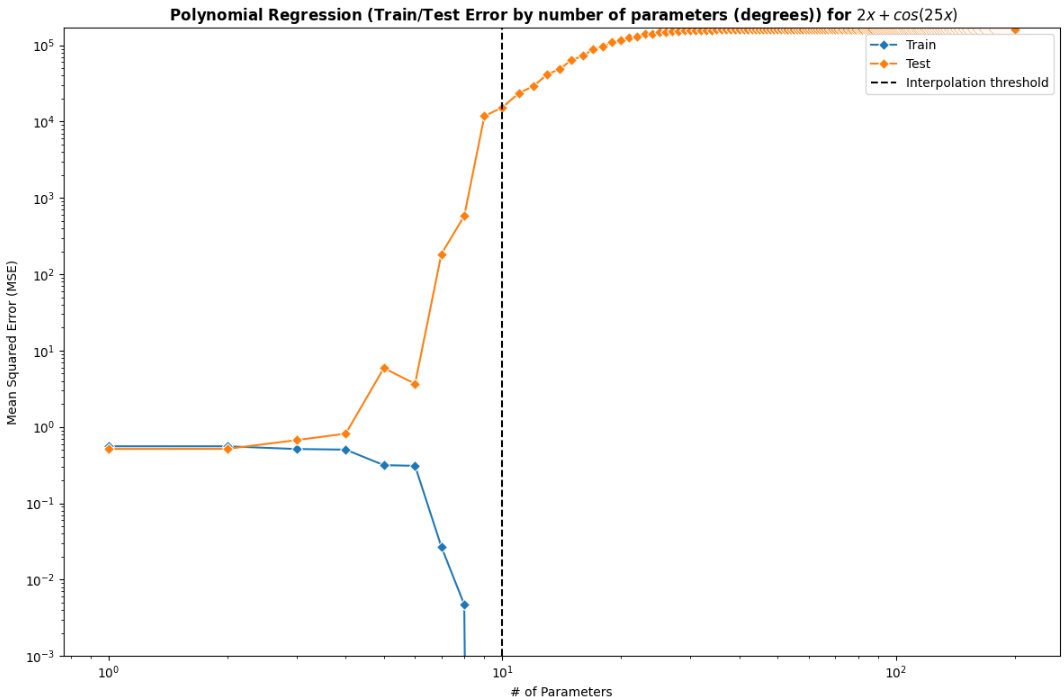
\includegraphics[width=\textwidth]{img/experiments/OLS1DDD.png}
        \caption{Error en entrenamiento y test para la aproximación polinómica clásica.}\label{fig:OLS1DDD}
    \end{subfigure}
    \hfill
    \begin{subfigure}[b]{0.48\textwidth}
        \centering
        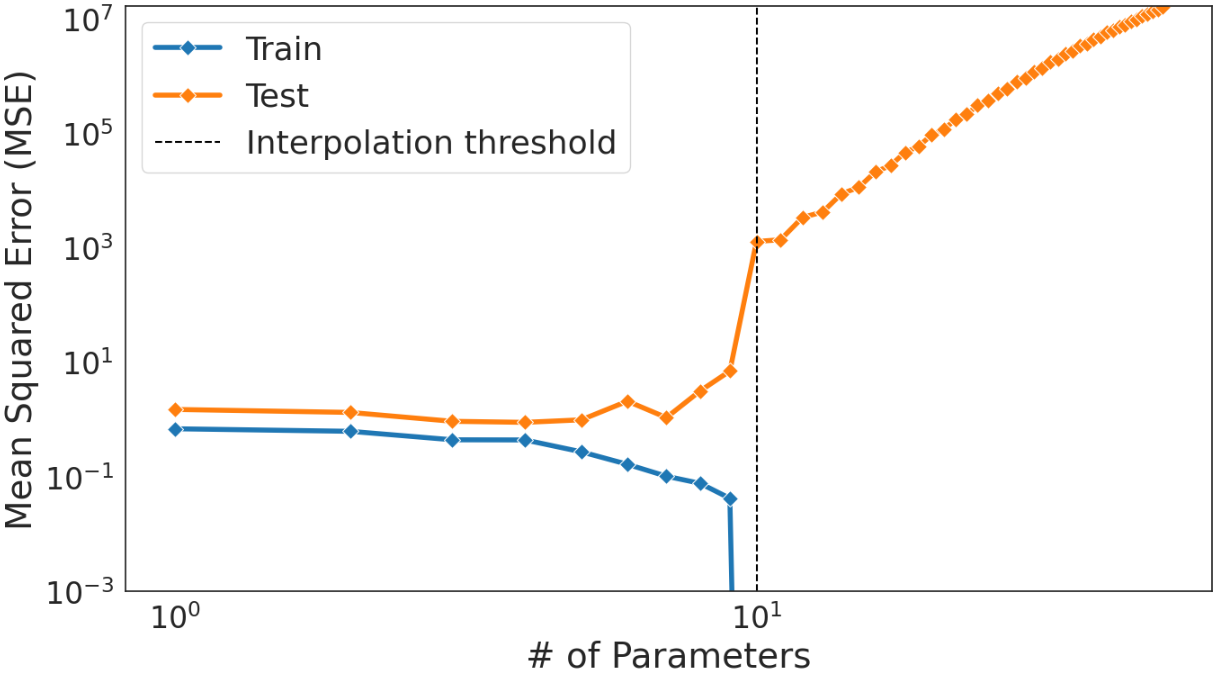
\includegraphics[width=\textwidth]{img/experiments/Redundant1DDD.png}
        \caption{Error en entrenamiento y test para la aproximación polinómica clásica redundante.}\label{fig:Redundant1DDD}
    \end{subfigure}
    \caption[Error en entrenamiento y test para las distintas aproximaciones polinómicas.]{Error en entrenamiento y test para la aproximación polinómica clásica y la redundante. El error en el conjunto de test se incrementa progresivamente.}\label{fig:aproximaciones-polinomicas}
\end{figure}

\begin{figure}[h]
    \centering
    \begin{subfigure}[b]{0.48\textwidth}
        \centering
        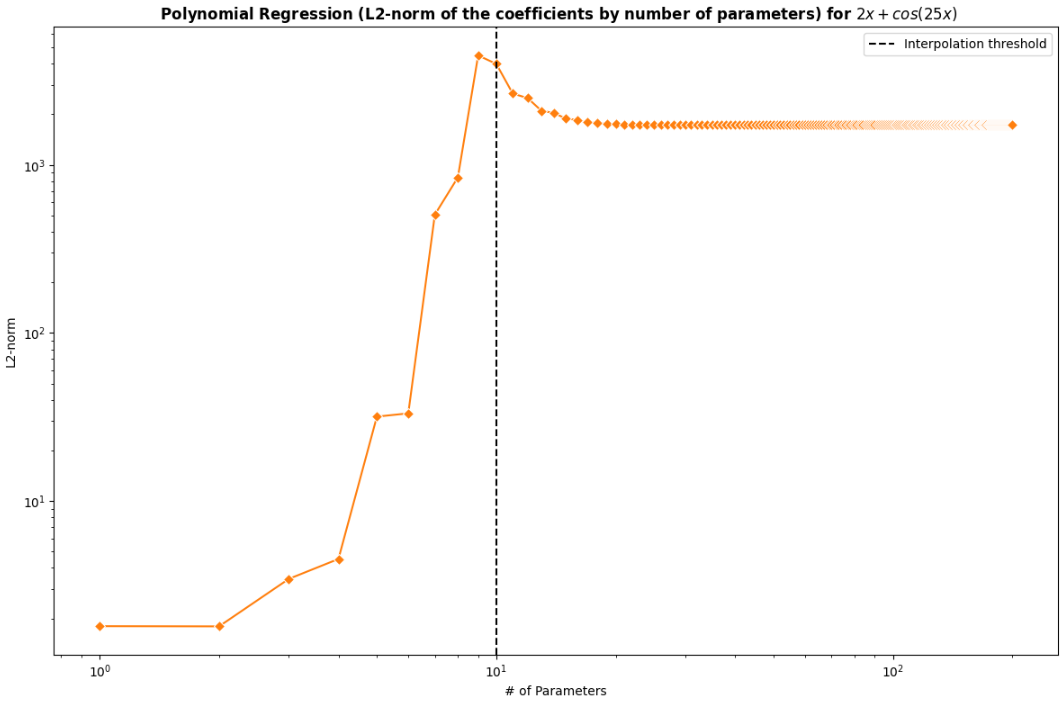
\includegraphics[width=\textwidth]{img/experiments/OLS1.4.png}
        \caption{Norma del vector de parámetros para la aproximación polinómica clásica.}\label{fig:OLS1.4DDD}
    \end{subfigure}
    \hfill
    \begin{subfigure}[b]{0.48\textwidth}
        \centering
        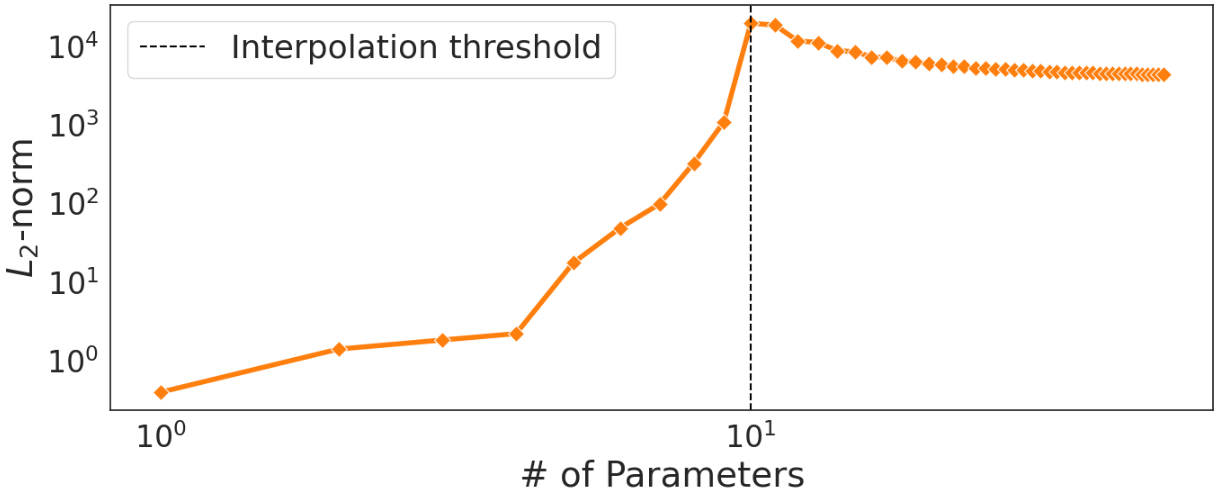
\includegraphics[width=\textwidth]{img/experiments/Redundant1.4.png}
        \caption{Norma del vector de parámetros para la aproximación polinómica clásica redundante.}\label{fig:Redundant1.4DDD}
    \end{subfigure}
    \caption[Normas del vector de parámetros para las aproximaciones polinómicas clásicas.]{Normas del vector de parámetros para las aproximaciones polinómicas clásicas. A medida que aumenta el número de parámetros, la norma del vector seleccionado es cada vez menor.}\label{fig:normas-clasicas}
\end{figure}

Finalmente, y de manera complementaria, se exponen en el Apéndice~\ref{ap:apendiceC} los resultados obtenidos al resolver este problema utilizando el descenso de gradiente como método de optimización, donde se observa la misma tendencia previamente descrita.

\begin{figure}[h]
    \centering
    \begin{minipage}{0.32\textwidth}
        \centering
        \textbf{Región infraparametrizada} \\[0.5ex] 
        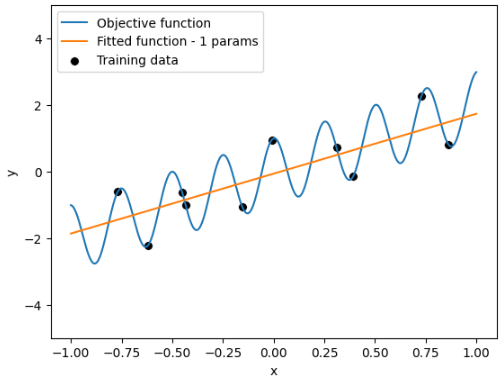
\includegraphics[width=\linewidth]{img/experiments/OLS1.1.png}
    \end{minipage}
    \begin{minipage}{0.32\textwidth}
        \centering
        \textbf{Umbral de interpolación} \\[0.5ex] 
        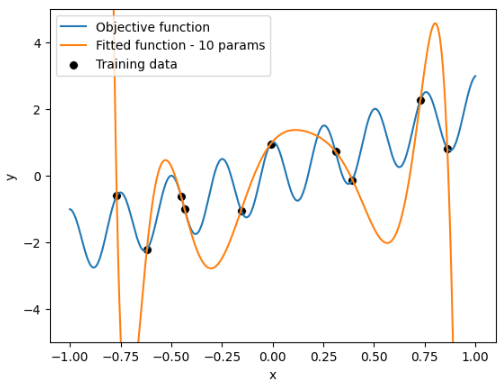
\includegraphics[width=\linewidth]{img/experiments/OLS1.2.png}
    \end{minipage}
    \begin{minipage}{0.32\textwidth}
        \centering
        \textbf{Región sobreparametrizada} \\[0.5ex] 
        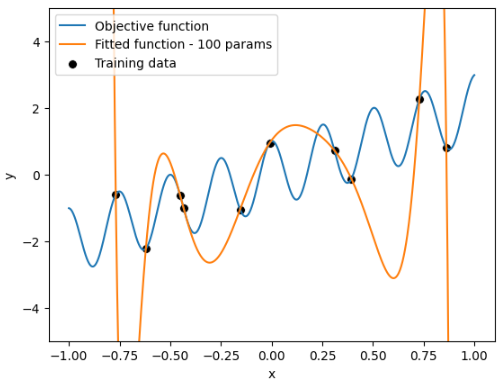
\includegraphics[width=\linewidth]{img/experiments/OLS1.3.png}
    \end{minipage}
    \caption[Aproximaciones polinómicas clásicas de la función objetivo.]{Aproximaciones polinómicas clásicas de la función objetivo. Se observa que, una vez superado el umbral de interpolación, añadir un mayor número de parámetros no contribuye a obtener una mejor aproximación.}\label{fig:polynomial1DD}
\end{figure}

La conclusión que podemos obtener de los resultados anteriores es que la base sobre la que estamos trabajando juega un papel fundamental en las aproximaciones obtenidas. De hecho, podemos considerar la base de Legendre, en cierta medida, como ``redundante'', dado que los polinomios que la conforman incluyen términos de polinomios anteriores. Por otro lado, la base polinomial clásica redundante se incorporó con la expectativa de que se reprodujera el fenómeno, debido también a su redundancia, sin embargo, no se reproduce. Esto sugiere que la base de Legendre, además de ser redundante, es más potente en características que no poseen las otras dos aproximaciones, lo que permite realizar aproximaciones progresivamente más precisas.

\subsubsection{Función hiperbólica}\label{subsubsec:funcion-hiperbolica}

Nos centramos ahora en trabajar con la aproximación de Legendre para una función objetivo cuya tendencia está dada por una función de tipo hiperbólica ($\tanh(x)$), y el ruido será determinado por la misma función que en la subsección anterior ($\cos(25x)$). Este experimento tiene como propósito verificar cómo el ruido contribuye a visualizar de manera más precisa el doble descenso.

\begin{figure}[h]
    \centering
    \begin{minipage}{0.32\textwidth}
        \centering
        \textbf{Región infraparametrizada} \\[0.5ex] 
        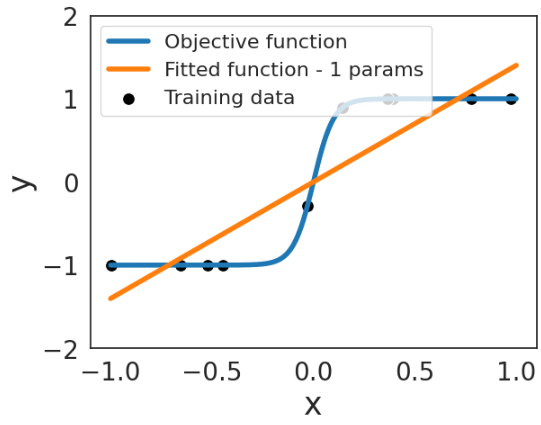
\includegraphics[width=\linewidth]{img/experiments/hiperbolica_noiseless1.1.png}
    \end{minipage}
    \begin{minipage}{0.32\textwidth}
        \centering
        \textbf{Umbral de interpolación} \\[0.5ex] 
        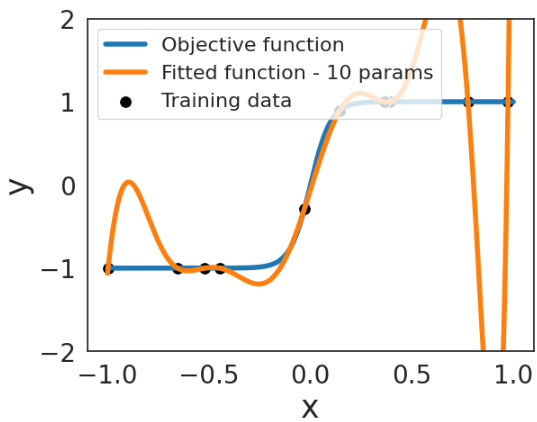
\includegraphics[width=\linewidth]{img/experiments/hiperbolica_noiseless1.2.png}
    \end{minipage}
    \begin{minipage}{0.32\textwidth}
        \centering
        \textbf{Región sobreparametrizada} \\[0.5ex] 
        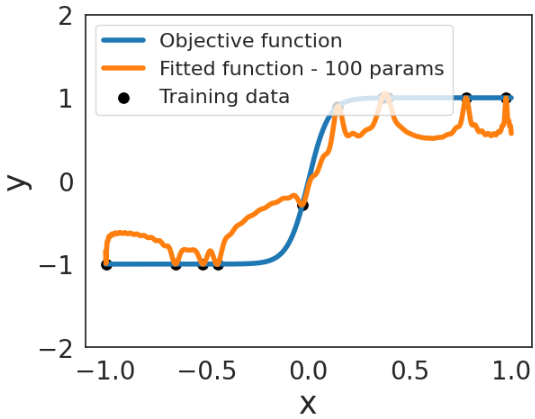
\includegraphics[width=\linewidth]{img/experiments/hiperbolica_noiseless1.3.png}
    \end{minipage} \\
    \begin{minipage}{0.32\textwidth}
        \centering
        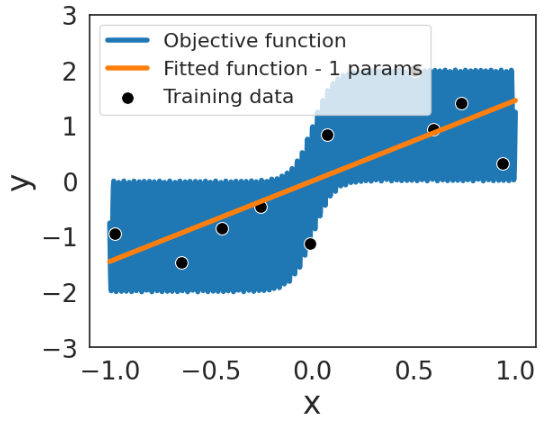
\includegraphics[width=\linewidth]{img/experiments/hiperbolica_noise1.1.png}
    \end{minipage}
    \begin{minipage}{0.32\textwidth}
        \centering
        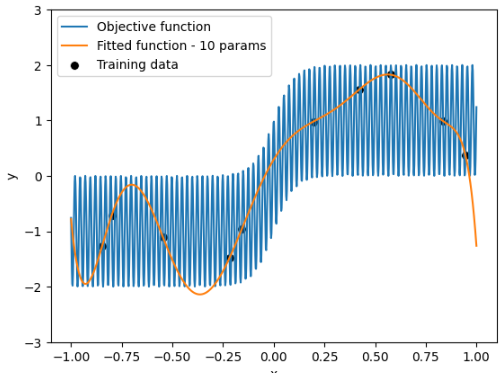
\includegraphics[width=\linewidth]{img/experiments/hiperbolica_noise1.2.png}
    \end{minipage}
    \begin{minipage}{0.32\textwidth}
        \centering
        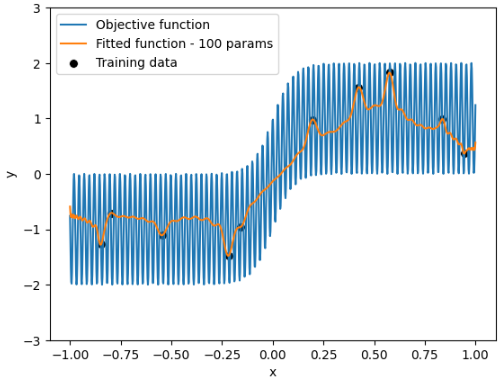
\includegraphics[width=\linewidth]{img/experiments/hiperbolica_noise1.3.png}
    \end{minipage}
    \caption[Aproximaciones polinómicas de Legendre de la función objetivo, tanto sin ruido como con ruido.]{Aproximaciones polinómicas de Legendre de la función objetivo, tanto sin ruido (fila superior) como con ruido (fila inferior). A medida que aumentan los parámetros, la predicción se ajusta y suaviza a la función objetivo.}\label{fig:approx-hiperbolicas}
\end{figure}

Para ello, usamos $10$ puntos muestreados de la función objetivo para el entrenamiento. En la Figura~\ref{fig:approx-hiperbolicas} podemos apreciar las distintas aproximaciones obtenidas por el modelo para el caso sin ruido y el caso con ruido, donde se puede observar cómo el aumento de parámetros ayuda a obtener mejores predicciones.

\begin{figure}[h]
    \centering
    \begin{subfigure}[b]{0.48\textwidth}
        \centering
        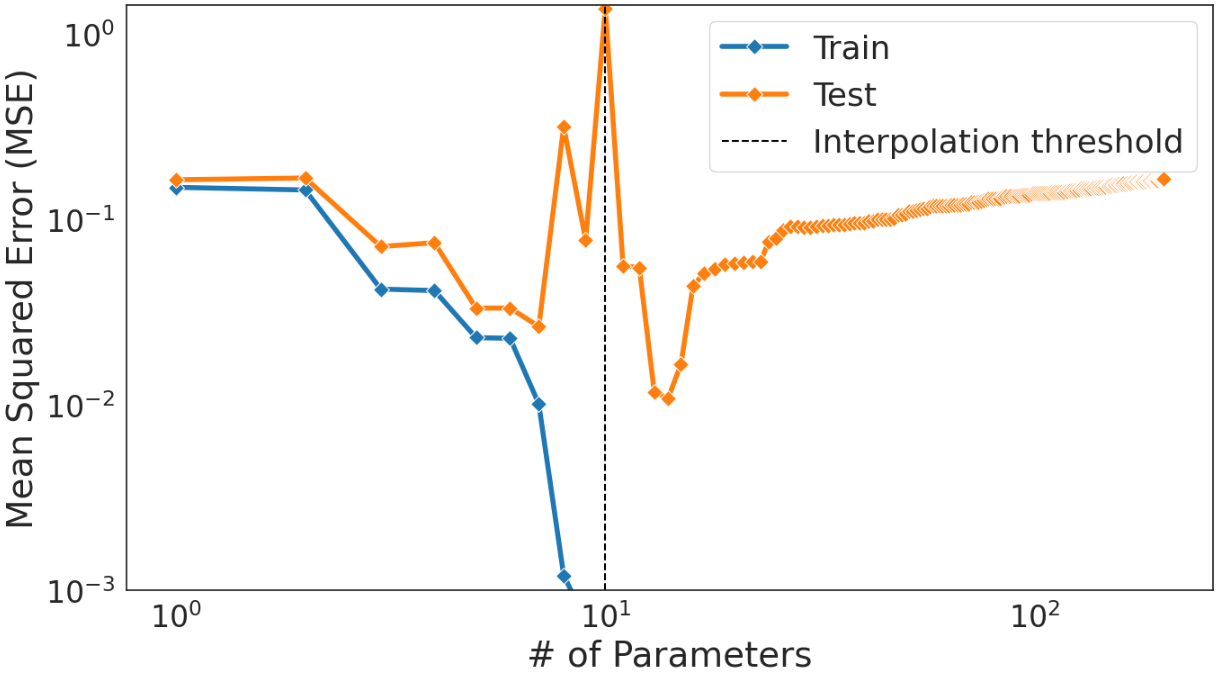
\includegraphics[width=\textwidth]{img/experiments/hiperbolica_noiselessDDD.png}
        \caption{Doble descenso para regresión polinómica de Legendre sin ruido.}\label{fig:hiperbolica_noiselessDDD}
    \end{subfigure}
    \hfill
    \begin{subfigure}[b]{0.48\textwidth}
        \centering
        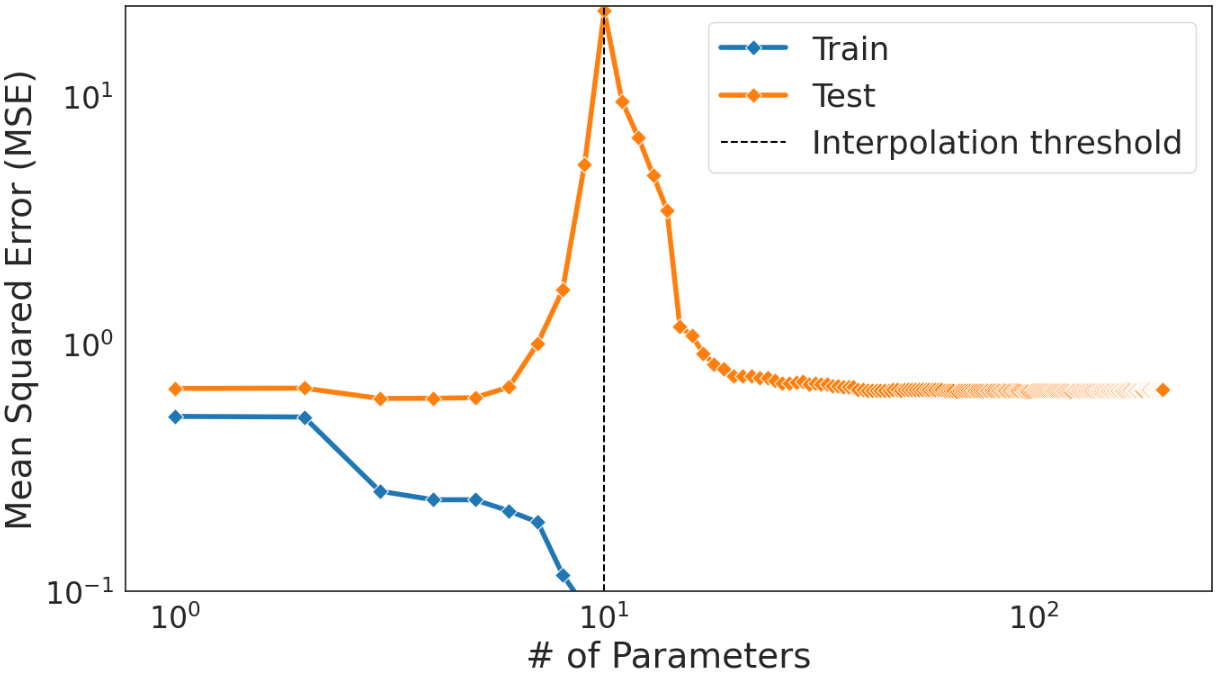
\includegraphics[width=\textwidth]{img/experiments/hiperbolica_noiseDDD.png}
        \caption{Doble descenso para regresión polinómica de Legendre con ruido.}\label{fig:hiperbolica_noiseDDD}
    \end{subfigure}
    \caption[Ejemplos de doble descenso en regresión polinómica de Legendre para una función objetivo, tanto con ruido como sin ruido.]{Ejemplos de doble descenso en regresión polinómica de Legendre para una función objetivo, tanto sin ruido como con ruido.}\label{fig:legendrehyperbolicDD}
\end{figure}

En la Figura~\ref{fig:legendrehyperbolicDD} podemos observar las curvas del error de test y entrenamiento para las distintas aproximaciones obtenidas en ambos casos. Destacamos el hecho de que, para el caso ruidoso, el doble descenso se presenta de forma más clara, donde al aumentar el número de parámetros se obtienen menores errores en el conjunto de test que los obtenidos durante el primer descenso. Este comportamiento va en consonancia con lo descrito en la literatura científica, donde al introducir ruido se observa el suceso con mayor claridad. Sumado a esto, las gráficas de la función objetivo ruidosa de la Figura~\ref{fig:approx-hiperbolicas} muestran cómo, al autoregulizarse el modelo y obtener una solución más simple, esta intenta suavizarse en torno al centro del conjunto de datos de entrenamiento, de modo que cualquier dato ruidoso no afecte excesivamente a la aproximación.

\subsubsection{Discusión}\label{subsubsec:discusion-polinomico}

Finalmente, para concluir este experimento, se presentan las principales conclusiones alcanzadas:

\begin{itemize}
    \item La base utilizada para la aproximación influye en la aparición del doble descenso, manifestándose al emplear la base de Legendre, pero no al utilizar las otras bases.
    \item Al aumentar el número de parámetros utilizados, la solución se ``autoregula'' hacia la solución de norma mínima del vector de parámetros, haciendo que la aproximación encontrada sea cada vez más suave, siguiendo la filosofía de Ockham.
    \item El ruido contribuye a obtener representaciones más claras del fenómeno, lo que resulta en errores de generalización menores que los obtenidos en el primer descenso. Esto sugiere que el modelo estaría identificando una forma de aislar ese ruido y centrarse en los datos realmente relevantes.
\end{itemize}

\subsection{\textit{Noise-wise double descent}}\label{subsec:noise-wise-dd}

En esta subsección, y como preámbulo al resto de experimentos, se estudia cómo varía el doble descenso al aumentar el porcentaje de ruido uniforme aleatorio en las etiquetas. De este modo, añadimos este tipo de doble descenso a las variantes clásicas propuestas por Nakkiran et al.\ en~\cite{Nakkiran2019}.

Para ello, se llevará a cabo un experimento con la arquitectura $2$NN sobre el dataset MNIST[$4000/1000$], modificando el porcentaje de ruido añadido en las etiquetas.

\begin{figure}[h]
    \centering
    \begin{minipage}{0.45\textwidth}
        \centering
        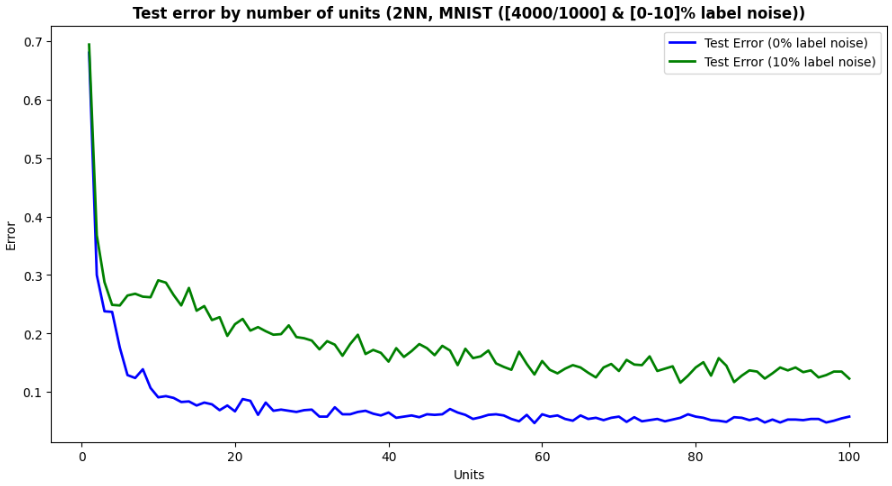
\includegraphics[width=\linewidth]{img/experiments/noise-wise-dd1.png}
    \end{minipage}
    \begin{minipage}{0.45\textwidth}
        \centering
        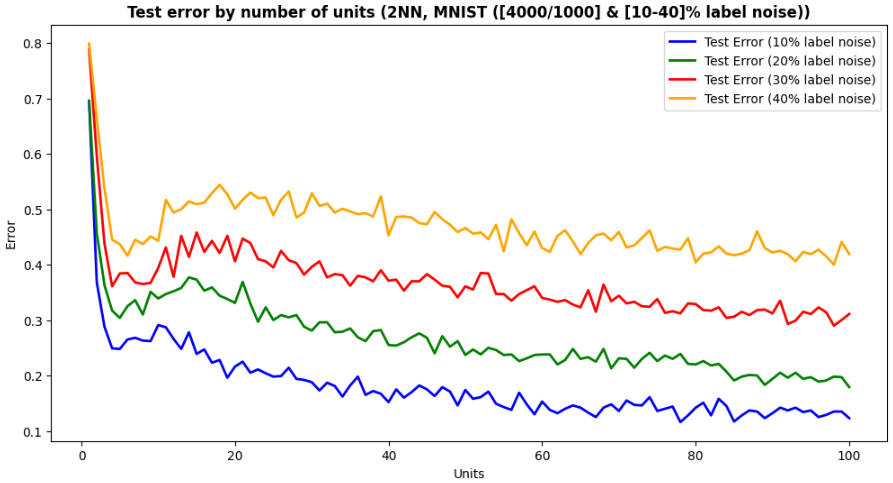
\includegraphics[width=\linewidth]{img/experiments/noise-wise-dd2.png}
    \end{minipage}
    \caption[Doble descenso para distintos niveles de ruido.]{Error en test de la arquitectura $2$NN sobre el subconjunto MNIST[$4000/1000$] para diferente nivel de ruido. A la izquierda, en ausencia de ruido añadido, el doble descenso no se manifiesta. En cambio, a la derecha, al aumentar el nivel de ruido, el pico de la curva se vuelve cada vez más pronunciado.}\label{fig:noise-wise-dd}
\end{figure}

En la Figura~\ref{fig:noise-wise-dd} se observa como un modelo que no presenta doble descenso sobre el conjunto de datos original sí lo experimenta al agregarle ruido. Además, en modelos donde si aparece el doble descenso, el pico del error de test aumenta al incrementar el porcentaje de ruido, lo que concuerda con lo conjeturado en la literatura científica, ya que el modelo, eventualmente, memorizará dicho ruido.

También se aprecia que, a medida que aumenta el ruido, se requieren más parámetros para alcanzar errores de test más bajos que el mínimo obtenido durante el primer descenso. Este fenómeno, junto con el aumento del tiempo de entrenamiento al incrementar el ruido (véase Tabla~\ref{tab:noisewisedd}) y considerando que, en escenarios reales, el porcentaje de ruido no suele ser excesivamente alto, nos lleva a optar por configuraciones con un nivel de ruido en torno al $10-20\%$ para los experimentos restantes.

Finalmente, en la Figura~\ref{fig:noise-wise-dd3} podemos verificar cómo, al aumentar el porcentaje de ruido en las etiquetas, el umbral de interpolación se desplaza hacia la derecha, lo que sugiere que los patrones que necesita aprender el modelo son más complejos a medida que aumentamos el ruido, siguiendo una lógica coherente. Además, este hecho pone de manifiesto que, en datos multidimensionales como las imágenes, se requieren más parámetros que el número de ejemplos utilizados. Esto es lógico, ya que una imagen no puede ser tratada como un objeto unidimensional, donde el umbral de interpolación permanece inalterado independientemente de la presencia de ruido, debido a que, para casos unidimensionales, siempre es posible memorizar un dato con un único parámetro (véase Figura~\ref{fig:legendre1DDD}).

\begin{figure}[h]
    \centering
    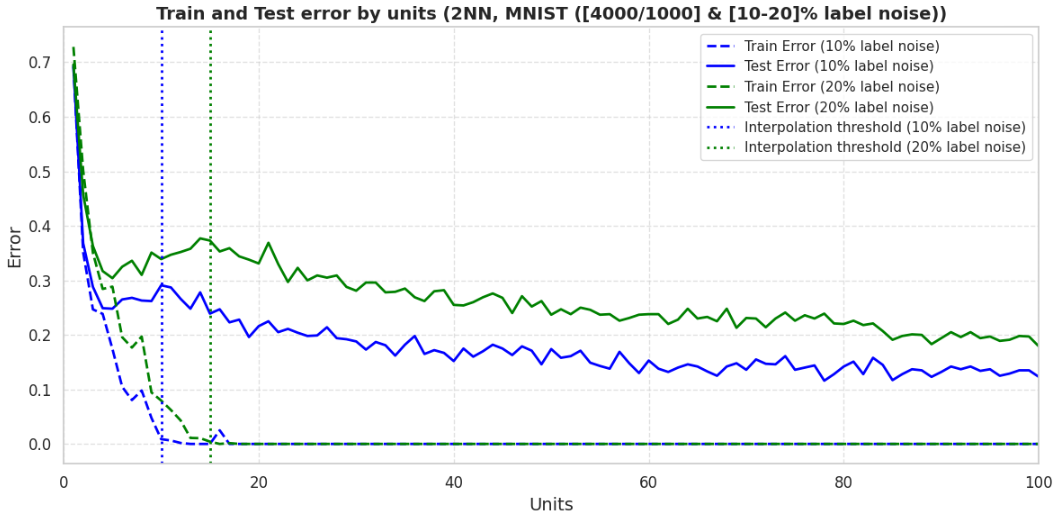
\includegraphics[width=0.45\textwidth]{img/experiments/noise-wise-dd3.png}
    \caption[Umbral de interpolación para el doble descenso con distintos niveles de ruido.]{Error en entrenamiento (línea discontinua), test (línea continua) y umbral de interpolación (línea punteada) respecto a la arquitectura $2$NN sobre el subconjunto MNIST[$4000/1000$] con distinto nivel de ruido añadido en las etiquetas.}\label{fig:noise-wise-dd3}
\end{figure}

\begin{table}[h!]
    \centering
    \begin{tabular}{|c|c|c|c|}
    \hline
    \textbf{Modelo}       & \textbf{Dataset} & \textbf{Ruido en etiquetas} & \textbf{Entrenamiento} \\ 
    \hline
    $2$NN ($1-100$)          & MNIST[$4000/1000$]        & $0\%$       & $26$h $10$min       \\ 
    $2$NN ($1-100$)          & MNIST[$4000/1000$]        & $10\%$         & $26$h $50$min       \\ 
    $2$NN ($1-100$)          & MNIST[$4000/1000$]        & $20\%$         & $27$h $23$min       \\ 
    $2$NN ($1-100$)          & MNIST[$4000/1000$]        & $30\%$          & $28$h $8$min       \\ 
    $2$NN ($1-100$)          & MNIST[$4000/1000$]       & $40\%$          & $30$h $14$min       \\  
    \hline
    \end{tabular}
    \caption[Resumen de los experimentos para el doble descenso por nivel de ruido.]{Resumen de los experimentos para el doble descenso por nivel de ruido.}
    \label{tab:noisewisedd}
\end{table}

\subsubsection{Discusión}\label{subsubsec:discusion-ruido}

En conclusión, a partir de los resultados obtenidos en este experimento, se presentan las siguientes conclusiones clave:

\begin{itemize}
    \item El ruido tiene un impacto significativo en la aparición del \textit{Deep Double Descent}, provocando que se pueda manifestar en conjuntos de datos donde, sin ruido, no ocurre.
    \item El ruido afecta al máximo error alcanzado, provocando un pico más pronunciado a medida que aumenta el nivel de ruido, relacionado con el hecho de que el modelo memoriza ese ruido.
    \item El ruido provoca un desplazamiento del umbral de interpolación hacia la derecha, ligado a que los patrones que el modelo debe aprender se vuelven más complejos.
\end{itemize}

\subsection{\textit{Sample-wise double descent}}\label{subsec:sample-wise-dd}

En esta subsección se presentan los experimentos realizados para analizar el impacto del tamaño del conjunto de datos sobre el doble descenso, conocido como \textit{sample-wise double descent}. Este efecto se manifiesta al modificar la cantidad de datos empleados para entrenar un modelo específico. Al comparar las curvas del error de generalización, se observa que entrenar con un mayor número de ejemplos puede, de manera casi paradójica\footnote{En el sentido que, generalmente, en el aprendizaje automático siempre se busca tener la mayor cantidad de datos posible de cara a entrenar.}, empeorar el rendimiento del modelo.

Dado que la experimentación presentada en la literatura existente resulta excesivamente costosa de replicar\footnote{Nakkiran et al.~\cite{Nakkiran2019} presentan este tipo de doble descenso utilizando Transformers (Figura 3) como modelo de procesamiento de lenguaje natural, incrementando su capacidad a través de su dimensión de incrustación (\textit{embedding}) y empleando un conjunto de datos de traducción automática.}, se han diseñado experimentos más accesibles que permiten analizarlo manteniendo un enfoque representativo. La idea para crear estos experimentos sencillos surge del hecho de que si un determinado modelo presenta \textit{model-wise doble descent} para un determinado número de ejemplos de entrenamiento, si aumentamos dicho número de ejemplos, el pico del error de test se desplazará hacia la derecha. Este desplazamiento da lugar a una región específica, a la que denominamos \textit{zona de interés}. Dentro de esta zona se verifica que entrenar con más ejemplos puede empeorar el rendimiento del modelo (véase la zona sombreada en color rojo de la Figura~\ref{fig:swdd}). Sin embargo, es importante resaltar que, fuera de esta zona, el incremento en la cantidad de ejemplos de entrenamiento suele tener un efecto positivo en el rendimiento del modelo, como nos dice la sabiduría clásica.

Por tanto, para la realización de este experimento se utilizará la red $2$NN, donde el número de unidades de salida de la primera capa densa variará desde $1$ hasta $200$. Además, se utilizará el dataset MNIST, sobre el que se extraeran $4000$ y $8000$ ejemplos para los distintos experimentos a realizar y a los que se les agregará un ruido del $10$\% en sus etiquetas.

\begin{figure}[h!]
    \centering
    \begin{minipage}{0.49\textwidth}
        \centering
        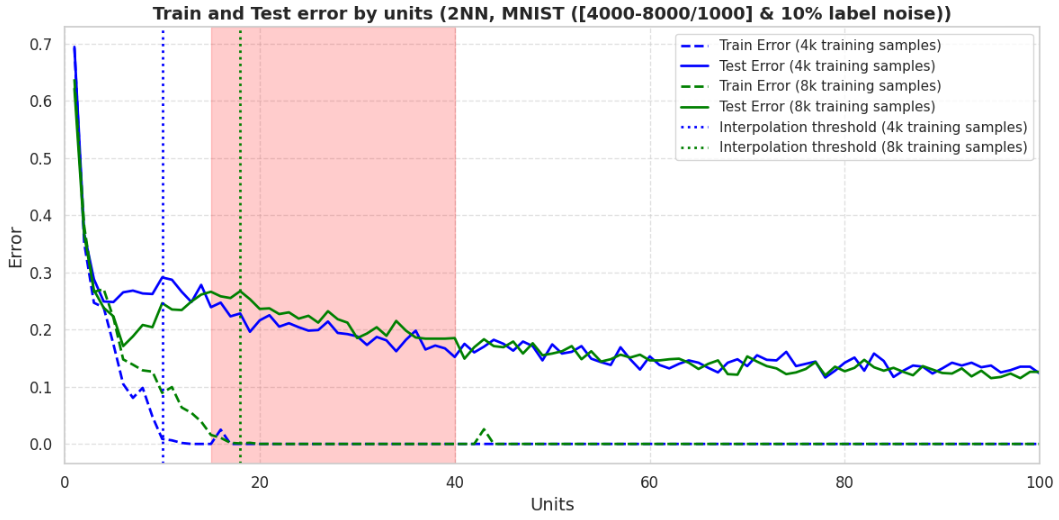
\includegraphics[width=\linewidth]{img/experiments/sample-wise-dd1.png}
    \end{minipage}
    \hfill
    \begin{minipage}{0.49\textwidth}
        \centering
        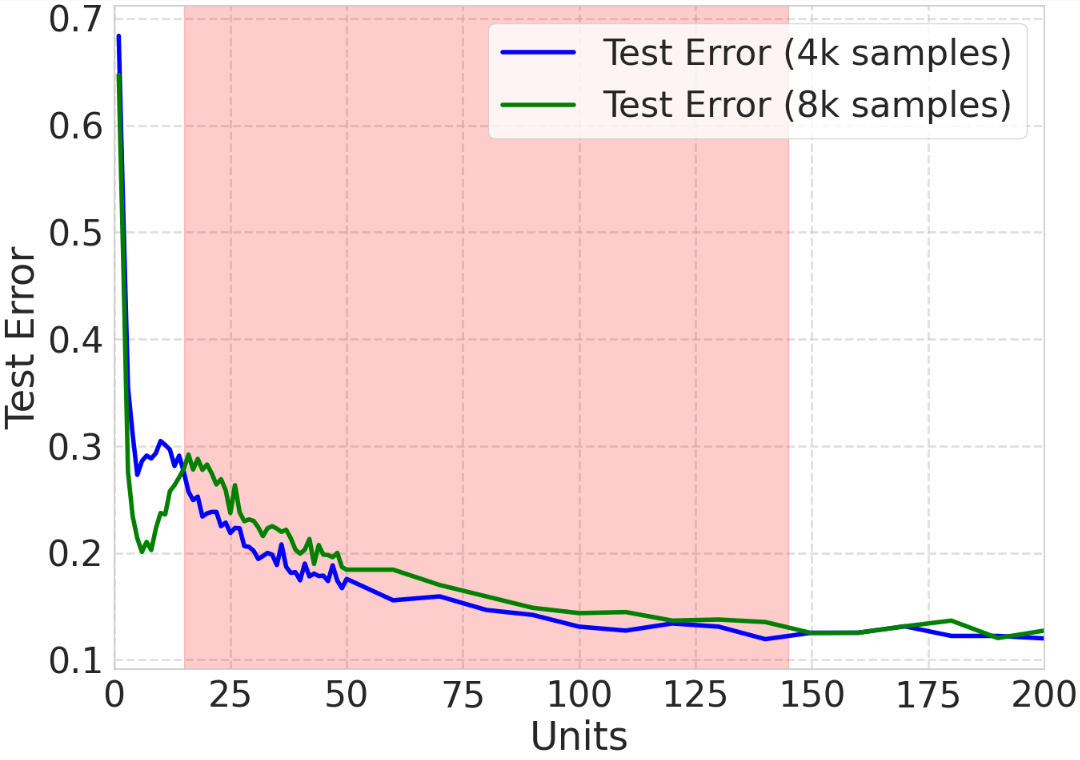
\includegraphics[width=\linewidth]{img/experiments/sample-wise-dd2.png}
    \end{minipage}
    \caption[Ejemplo de \textit{sample-wise double descent}.]{Ejemplo de \textit{sample-wise double descent} para la red $2$NN sobre dos subconjuntos de MNIST con $10\%$ de ruido añadido, utilizando $4000$ y $8000$ ejemplos de entrenamiento. A la izquierda aparece el resultado de una única realización del experimento. A la derecha aparece el resultado obtenido al realizar la media de $3$ experimentos. Se puede observar cómo, con el doble de datos (línea verde), no solo el punto de interpolación se desplaza a la derecha (apareciendo más tarde), sino también el error de test es, en la mayor parte de casos, menor cuando se emplean menos ejemplos de entrenamiento.}\label{fig:swdd}
\end{figure}

Al igual que ocurría al aumentar el nivel de ruido, si aumentamos el número de ejemplos de entrenamiento, el umbral de interpolación también se desplaza hacia la derecha (véase Figura~\ref{fig:swdd}). Es decir, el modelo requiere de un mayor número de parámetros para memorizar un mayor número de ejemplos de entrenamiento, lo que, en principio, resulta coherente con la complejidad efectiva del modelo y con la propia lógica humana.

Finalmente, se muestra en la Tabla~\ref{tab:model_training_time} el tiempo de ejecución necesario para la realización de este experimento. Cabe destacar que, en el experimento donde se calcula la media de $3$ ejecuciones, se utiliza el modelo $2$NN hasta $50$ unidades (de $1$ en $1$) y, a partir de este valor, se suman las unidades de $10$ en $10$ hasta llegar a $200$ unidades, con el propósito de acelerar el entrenamiento fuera de la zona de interés que proporcionaba el primer experimento.

\begin{table}[h!]
\centering
\begin{tabular}{|c|c|c|}
\hline
\textbf{Modelo}       & \textbf{Dataset} & \textbf{Entrenamiento} \\ 
\hline
$2$NN ($1-100$)      & MNIST[$4000/1000$] ($10$\% label noise)        & $26$h $50$min       \\ 
$2$NN ($1-100$)      & MNIST[$8000/1000$]  ($10$\% label noise)       & $59$h       \\ 
$2$NN ($1-200$) $\times$ $3$     & MNIST[$4000/1000$]  ($10$\% label noise)       & $53$h $10$min       \\ 
$2$NN ($1-200$) $\times$ $3$      & MNIST[$8000/1000$]  ($10$\% label noise)       & $104$h $30$min       \\ 
$2$NN ($1-100$)          & MNIST[$12000/1000$] ($10$\% label noise)   & $65$h $50$min   \\ 
$2$NN ($1-100$)          & MNIST[$16000/1000$] ($10$\% label noise)   & $102$h $49$min   \\ 
\hline
\end{tabular}
\caption[Resumen de los experimentos para el doble descenso por número de ejemplos de entrenamiento.]{Resumen de los experimentos para el doble descenso por número de ejemplos de entrenamiento.}\label{tab:model_training_time}
\end{table}

\subsubsection{Ratio parámetros/ejemplos}\label{subsubsec:ratio-parametros-ejemplos}

En este apartado, se analiza la relación entre el número de parámetros y el número de ejemplos con el objetivo de estudiar la tendencia del umbral de interpolación en función de este cociente. Para ello, se lleva a cabo un experimento utilizando la arquitectura $2$NN sobre el dataset MNIST, variando la cantidad de ejemplos de entrenamiento. Además, se introduce un $10\%$ de ruido en las etiquetas.

\begin{figure}[h]
    \centering
    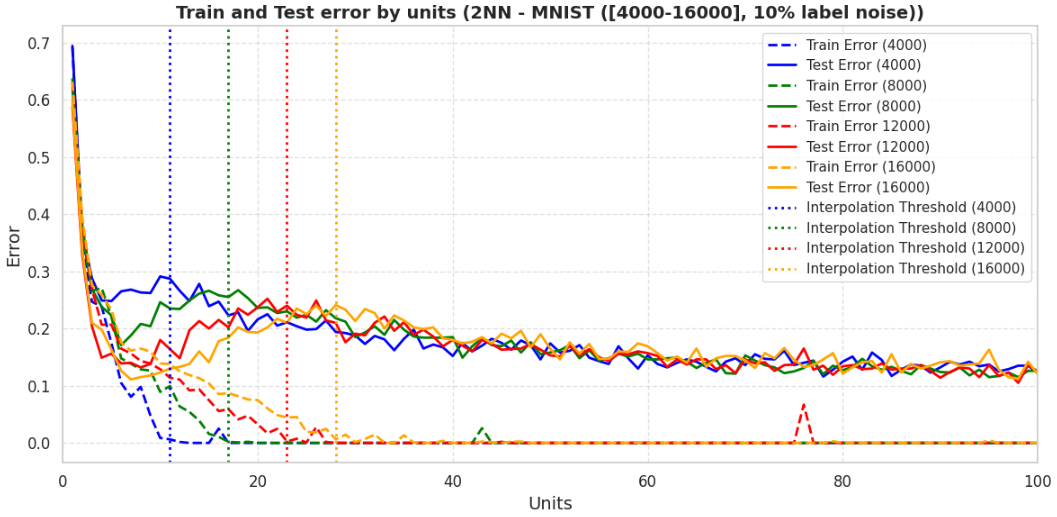
\includegraphics[width=0.5\textwidth]{img/experiments/ratioparamsexamples.png}
    \caption[Ratio parámetros frente a número de ejemplos en el doble descenso.]{Error en entrenamiento (línea discontinua) y prueba (línea continua) de la arquitectura $2$NN sobre el dataset MNIST[$4000-16000$] y $10$\% de ruido añadido a las etiquetas. Además, se muestra el umbral de interpolación (línea punteada) para cada número de ejemplos.}\label{fig:ratioparamsexamples}
\end{figure}

La Figura~\ref{fig:ratioparamsexamples} confirma nuevamente, como se mencionó previamente, que al aumentar el número de ejemplos de entrenamiento, el umbral de interpolación se desplaza hacia la derecha. Asimismo, este experimento valida que dicho máximo se produce cuando el modelo alcanza un error de entrenamiento cercano a cero, en correspondencia con la noción de complejidad efectiva.

No obstante, a partir de este experimento también es posible extraer conclusiones sobre el ratio entre parámetros y ejemplos en el que aparece dicho umbral de interpolación, lo que permite estudiar su comportamiento a medida que ambos aumentan. A partir de los datos presentados en la Tabla~\ref{tab:ratioparamsexamples}, se observa que el cociente entre el número de parámetros y el número de ejemplos en el que se alcanza el umbral de interpolación tiende a decrecer a medida que aumenta la cantidad de datos de entrenamiento. Este comportamiento sugiere que, en el límite de un número suficientemente grande de ejemplos, dicho ratio se aproxima progresivamente a uno, indicando una relación más equilibrada entre la capacidad del modelo y la cantidad de datos necesarios para alcanzar el régimen de interpolación. 

Finalmente, los tiempos de entrenamiento correspondientes a este experimento se muestran en la Tabla~\ref{tab:model_training_time}. Se destaca el notable incremento en el tiempo de entrenamiento a medida que aumenta el número de ejemplos, lo que limita la viabilidad de un análisis más exhaustivo sobre la convergencia de este cociente.

\begin{table}[h]
    \centering
    \begin{tabular}{|c|c|c|c|}
    \hline
    \textbf{Modelo}       & \textbf{Número de parámetros} & \textbf{Ejemplos} & \textbf{Ratio} \\ 
    \hline
    $2$NN ($11$)          & $8755$   & $4000$  &  $\approx$ $2,19$  \\ 
    $2$NN ($17$)          & $13525$   & $8000$  &  $\approx$ $1,69$  \\ 
    $2$NN ($23$)          & $18295$   & $12000$  &  $\approx$ $1,52$  \\ 
    $2$NN ($28$)          & $22270$   & $16000$  &  $\approx$ $1,39$  \\ 
    \hline
    \end{tabular}
    \caption[Resumen del ratio parámetros/ejemplos.]{Ratio de parámetros/ejemplos relativo al umbral de interpolación para diferentes cantidades de ejemplos de entrenamiento.}\label{tab:ratioparamsexamples}
\end{table}

\subsubsection{Discusión}\label{subsubsec:discusion-numero-ejemplos}

Para cerrar este experimento, se exponen las conclusiones más relevantes alcanzadas:

\begin{itemize}
    \item Al aumentar el número de ejemplos, el umbral de interpolación se desplaza hacia la derecha, dado que el modelo requiere más capacidad para alcanzar su complejidad efectiva. Esto da lugar a una zona en la que, de manera paradójica, entrenar con un mayor número de ejemplos empeora el rendimiento.
    \item Se calcula, mediante un ejemplo sencillo, el promedio entre el número de parámetros y los ejemplos en los que aparece el umbral, y se observa que sigue una tendencia decreciente hasta converger, aparentemente, hacia el valor de $1$.
\end{itemize}

\subsection{\textit{Model \& Epoch-wise double descent}}\label{subsec:model-epoch-wise}

Nos centramos ahora en la verificación del \textit{Deep Double Descent} en sus dos versiones más comunes: el doble descenso en función de la complejidad del modelo (\textit{model-wise}) y en función del número de épocas (\textit{epoch-wise}). A tal efecto, representaremos ambos comportamientos de manera conjunta en una gráfica que muestra el número de parámetros en el eje $X$ y el número de épocas en el eje $Y$. De este modo, el \textit{model-wise double descent} se puede observar al fijar el eje $Y$, mientras que el \textit{epoch-wise double descent} se visualiza al fijar el eje $X$. Además, esta representación permite analizar la tendencia que sigue el umbral de interpolación en función del cociente entre el número de épocas y el número de parámetros.

\subsubsection{2NN}\label{subsubsec:model-epoch-wise-2NN}

En primer lugar, trabajaremos con la arquitectura $2$NN debido a su baja capacidad. Para garantizar que esta arquitectura cuente con un número de parámetros superior al de ejemplos y, al mismo tiempo, acelerar el entrenamiento, usaremos subconjuntos de $4000$ ejemplos de entrenamiento extraídos de los conjuntos de datos utilizados.

\begin{figure}[h]
    \centering
    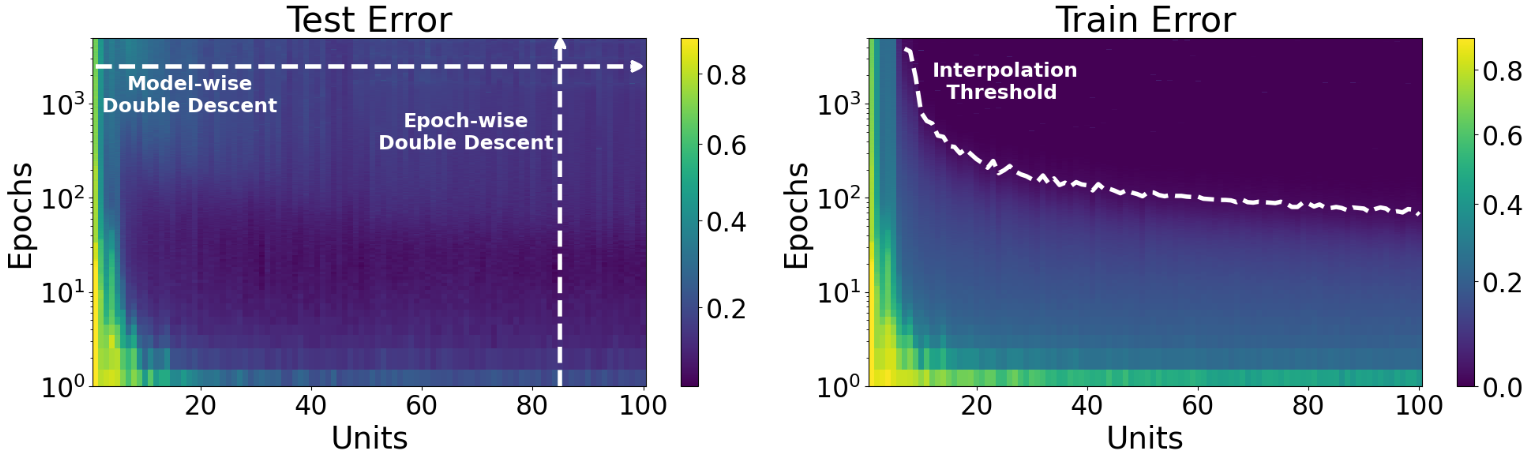
\includegraphics[width=0.95\textwidth]{img/experiments/model-epoch2NNMNIST.png}
    \caption[Doble descenso en función del tamaño del modelo y del número de épocas para la red $2$NN y un subconjunto de MNIST.]{A la izquierda se muestra el error de test en función del tamaño del modelo y del número de épocas de entrenamiento. A la derecha, se representa el error de entrenamiento de los modelos correspondientes. Todas las arquitecturas consideradas son redes $2$NN entrenadas en el subconjunto MNIST[$4000/1000$], con $10\%$ de ruido añadido y durante $5000$ épocas. Se puede observar que, en términos globales, a mayor número de unidades (eje $X$) y mayor número de épocas (eje $Y$), mejores resultados a nivel de \textit{accuracy} en test (colores más oscuros). Más concretamente, hay una franja entre $5$ y $10^2$ épocas en donde parece que se acumulan los mejores resultados del primer descenso.}\label{fig:model-epoch2NNMNIST}
\end{figure}

La Figura~\ref{fig:model-epoch2NNMNIST} muestra de manera clara ambos tipos de doble descenso. Por otra parte, en la imagen de la derecha se muestra el umbral de interpolación (punto en el que el modelo obtiene un error de entrenamiento cercano a $0$), donde podemos observar como el cociente épocas/parámetros sigue una tendencia decreciente hasta estabilizarse, algo similar a lo que ocurre con el ratio parámetros/ejemplos (véase Subsección~\ref{subsubsec:ratio-parametros-ejemplos}). Este resultado sugiere que, a medida que el tamaño del modelo aumenta, el número de épocas necesarias para alcanzar el umbral de interpolación se reduce de forma progresiva, hasta alcanzar un régimen en el que este cociente se mantiene prácticamente constante. Dicho comportamiento refuerza la idea de que la interpolación se vuelve más eficiente en términos de entrenamiento cuando la capacidad del modelo es suficientemente grande.

\begin{figure}[h]
    \centering
    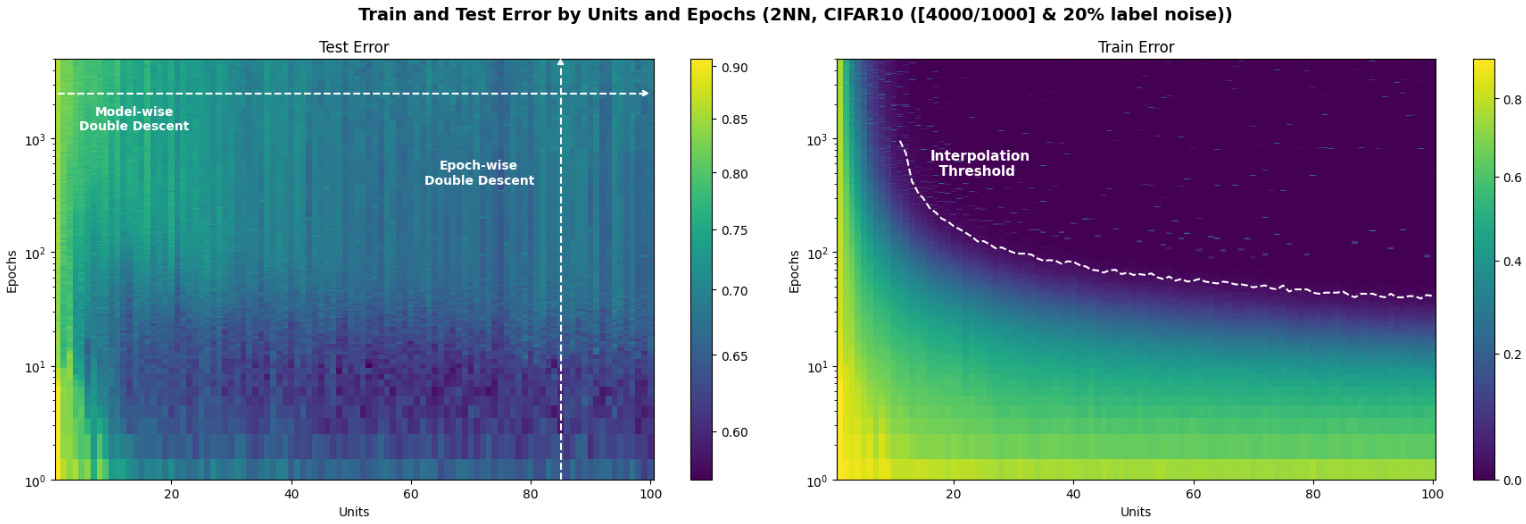
\includegraphics[width=0.95\textwidth]{img/experiments/model-epoch2NNCIFAR10.png}
    \caption[Error en entrenamiento y test en función del tamaño del modelo y del número de épocas para la red $2$NN y un subconjunto de CIFAR$10$.]{A la izquierda se muestra el error en test en función del tamaño del modelo y del número de épocas de entrenamiento. A la derecha, se representa el error de entrenamiento de los modelos correspondientes. Todas las arquitecturas consideradas son redes $2$NN entrenadas en el subconjunto CIFAR$10$[$4000/1000$], con $20\%$ de ruido añadido, durante $5000$ épocas y con un \textit{batch size} de $128$. Los resultados obtenidos en este experimento son peores a los del conjunto de datos anterior, lo cual puede atribuirse a que la arquitectura presenta una complejidad insuficiente, lo que limita su capacidad de generalización.}\label{fig:model-epoch2NNCIFAR10}
\end{figure}

Por otro lado, la Figura~\ref{fig:model-epoch2NNCIFAR10} no muestra, al menos de forma tan evidente, el doble descenso en el conjunto de datos CIFAR$10$. Esto sugiere que, aunque se ha utilizado la misma cantidad de datos, la mayor complejidad de este conjunto (al tratarse de imágenes en formato RGB) implica que la arquitectura $2$NN no posee la capacidad suficiente para manifestar dicho comportamiento. Debido a este resultado, se decide no realizar el experimento con el conjunto de datos CIFAR$100$, ya que se anticipa un resultado igualmente desfavorable, dado que ambos conjuntos comparten el mismo formato de imágenes (véase Tabla~\ref{tab:datasets}).

Finalmente, en la Tabla~\ref{tab:2nn_model-epochwise} se recogen los tiempos de entrenamiento requeridos para la realización de este experimento.

\begin{table}[h!]
    \centering
    \begin{tabular}{|c|c|c|}
    \hline
    \textbf{Modelo}       & \textbf{Dataset} & \textbf{Entrenamiento} \\ 
    \hline
    $2$NN ($1-100$)      & MNIST[$4000/1000$] ($10$\% label noise)        & $179$h $5$min \\ 
    $2$NN ($1-100$)      & CIFAR$10$[$4000/1000$]  ($20$\% label noise)   & $213$h $32$min \\
    \hline
    \end{tabular}
    \caption[Resumen de los experimentos para el doble descenso por complejidad del modelo y épocas para la red $2$NN.]{Resumen de los experimentos para el doble descenso por complejidad del modelo y épocas para la red $2$NN.}\label{tab:2nn_model-epochwise}
\end{table}

\subsubsection{3CNN}\label{subsubsec:model-epoch-wise-3CNN}

Continuamos con los experimentos realizados para la arquitectura $3$CNN, la cual es más potente que la arquitectura $2$NN debido a su mayor número de parámetros y a la inclusión de bloques convolucionales, que facilitan la extracción de características de las imágenes. Es por esto que, para la realización de estos experimentos, se considerarán subconjuntos de datos con un mayor número de ejemplos que en el apartado anterior.

\begin{figure}[h]
    \centering
    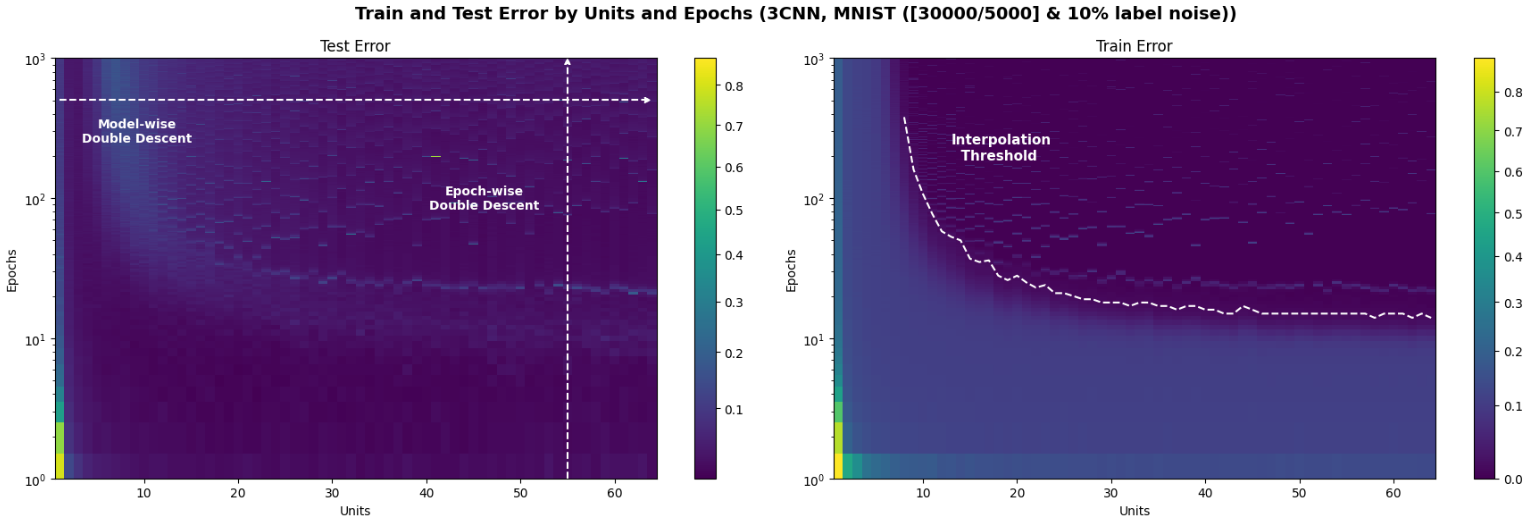
\includegraphics[width=0.95\textwidth]{img/experiments/model-epoch3CNNMNIST30k.png}
    \caption[Doble descenso en función del tamaño del modelo y del número de épocas para la red $3$CNN y un subconjunto de MNIST.]{A la izquierda se muestra el error en prueba en función del tamaño del modelo y del número de épocas de entrenamiento. A la derecha, se representa el error de entrenamiento de los modelos correspondientes. Todas las arquitecturas consideradas son redes $3$CNN entrenadas en el subconjunto MNIST[$30000/5000$], con $10\%$ de ruido añadido y con un \textit{batch size} de $128$.}\label{fig:model-epoch3CNNMNIST30k}
\end{figure}

La Figura~\ref{fig:model-epoch3CNNMNIST30k} muestra con claridad ambos tipos de doble descenso sobre un subconjunto del conjunto de datos MNIST. Asimismo, se observa que el error obtenido para esta arquitectura es menor que el de la arquitectura anterior, lo que es coherente con su mayor capacidad.

Por otra parte, las Figuras~\ref{fig:model-epoch3CNNCIFAR10} y~\ref{fig:model-epoch3CNNCIFAR10025k} también muestran ambos tipos de doble descenso, aunque de forma menos evidente y con variaciones abruptas tanto en el error de entrenamiento como en el de test sobre dos subconjutos de datos de CIFAR$10$ y CIFAR$100$. Estos saltos se analizan con más detalle en el Apéndice~\ref{ap:apendiceD}. Asimismo, el error obtenido es mayor, dado que trabajamos con imágenes en formato RGB y de mayor dimensionalidad. Finalmente, la Tabla~\ref{tab:3cnn_model-epochwise} recoge los tiempos de entrenamiento requeridos para la realización de este experimento.

\begin{figure}[h]
    \centering
    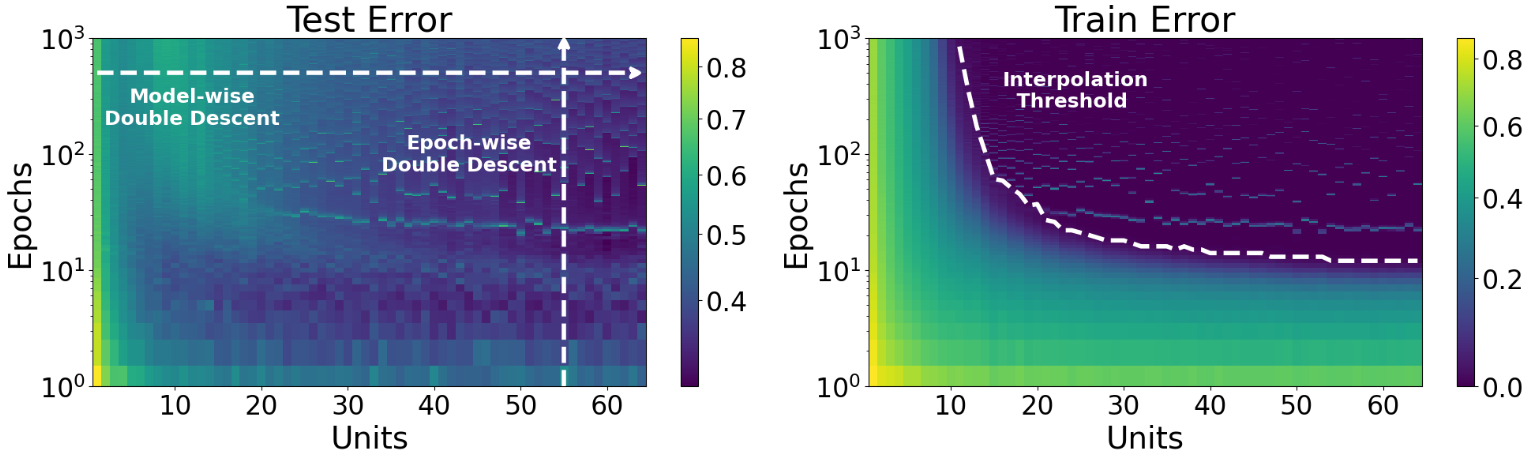
\includegraphics[width=0.95\textwidth]{img/experiments/model-epoch3CNNCIFAR1025k.png}
    \caption[Doble descenso en función del tamaño del modelo y del número de épocas para la red $3$CNN y un subconjunto de CIFAR$10$.]{A la izquierda se muestra el error en prueba en función del tamaño del modelo y del número de épocas de entrenamiento. A la derecha, se representa el error de entrenamiento de los modelos correspondientes. En ambas gráficas se identifican regiones donde el error experimenta repuntes de forma transitoria. Todas las arquitecturas consideradas son redes $3$CNN entrenadas en el subconjunto CIFAR$10$[$25000/5000$], con $20\%$ de ruido añadido y con un \textit{batch size} de $128$.}\label{fig:model-epoch3CNNCIFAR10}
\end{figure}

\begin{figure}[h]
    \centering
    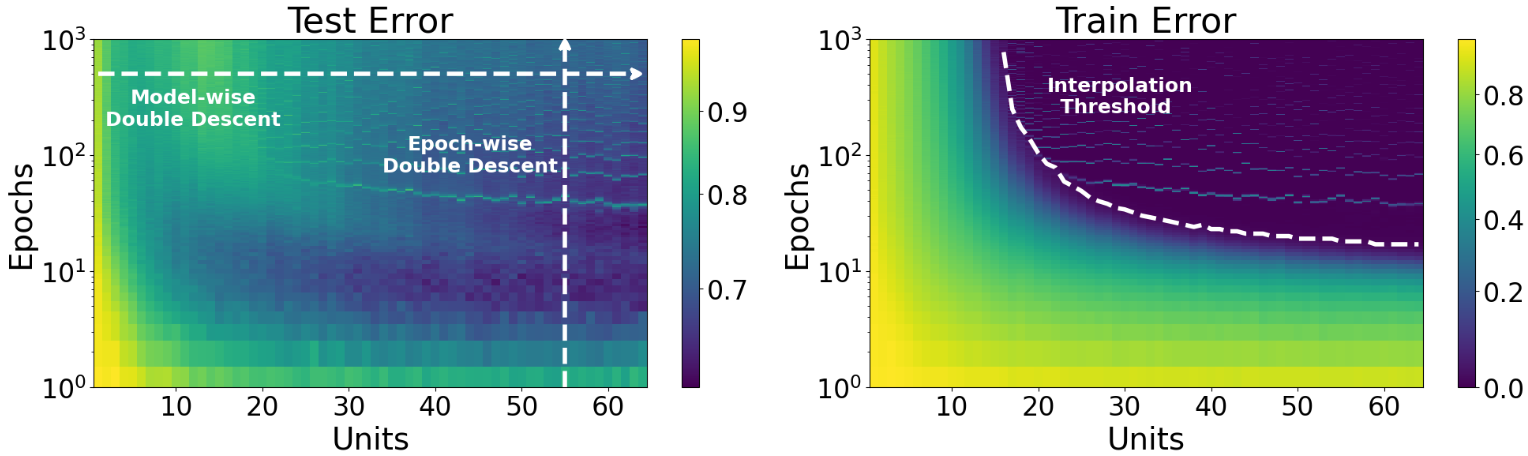
\includegraphics[width=0.95\textwidth]{img/experiments/model-epoch3CNNCIFAR10025k.png}
    \caption[Doble descenso en función del tamaño del modelo y del número de épocas para la red $3$CNN y un subconjunto de CIFAR$100$.]{A la izquierda se muestra el error en prueba en función del tamaño del modelo y del número de épocas de entrenamiento. A la derecha, se representa el error de entrenamiento de los modelos correspondientes. En ambas gráficas se identifican regiones donde el error experimenta repuntes de forma transitoria. Todas las arquitecturas consideradas son redes $3$CNN entrenadas en el subconjunto CIFAR$100$[$25000/5000$], con $20\%$ de ruido añadido y con un \textit{batch size} de $128$.}\label{fig:model-epoch3CNNCIFAR10025k}
\end{figure}

\begin{table}[h!]
    \centering
    \begin{tabular}{|c|c|c|}
    \hline
    \textbf{Modelo}       & \textbf{Dataset} & \textbf{Entrenamiento} \\ 
    \hline
    $3$CNN ($1-64$)      & MNIST[$30000/5000$] ($10$\% label noise)        & $179$h $5$min \\ 
    $3$CNN ($1-64$)      & CIFAR$10$[$25000/5000$]  ($20$\% label noise)   & $147$h $11$min \\
    $3$CNN ($1-64$)      & CIFAR$100$[$25000/5000$]  ($20$\% label noise)   & $152$h $56$min \\
    \hline
    \end{tabular}
    \caption[Resumen de los experimentos para el doble descenso por complejidad del modelo y épocas para la arquitectura $3$CNN.]{Resumen de los experimentos para el doble descenso por complejidad del modelo y épocas para la arquitectura $3$CNN.}\label{tab:3cnn_model-epochwise}
\end{table}

\subsubsection{ResNet18 modificada}\label{subsubsec:model-epoch-wise-ResNet18 modificada}

Finalmente, se presentan los experimentos realizados con la arquitectura ResNet$18$ modificada, la cual posee el mayor número de parámetros entre las arquitecturas consideradas en este estudio. Dada su mayor capacidad de representación, se utilizan los conjuntos de datos en su totalidad para aprovechar al máximo su potencial.

Sin embargo, estos experimentos se vieron condicionados por la limitación impuesta por la Universidad de Granada en cuanto al tiempo máximo de uso de los nodos de cómputo. Como consecuencia, el número de épocas de entrenamiento se redujo de forma significativa, lo que ha afectado de manera significativa a la precisión de los resultados obtenidos.

\begin{figure}[h]
    \centering
    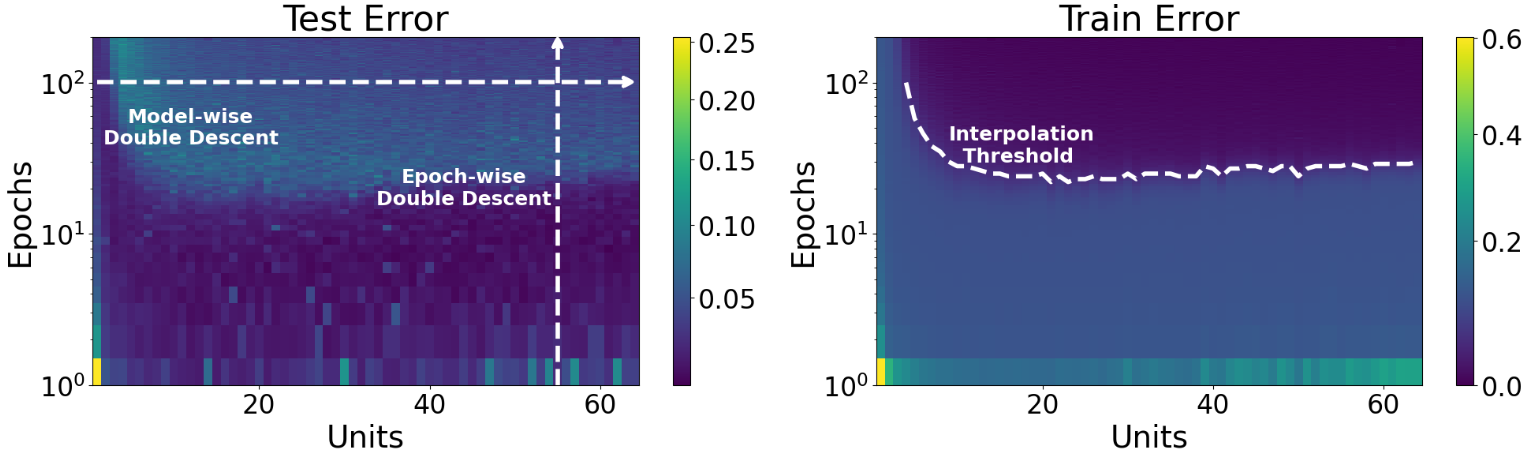
\includegraphics[width=0.95\textwidth]{img/experiments/model-epochPreActResNet18MNIST.png}
    \caption[Doble descenso en función del tamaño del modelo y del número de épocas para la red ResNet$18$ y el conjunto MNIST.]{A la izquierda se muestra el error en prueba en función del tamaño del modelo y del número de épocas de entrenamiento. A la derecha, se representa el error de entrenamiento de los modelos correspondientes. Todas las arquitecturas consideradas son redes ResNet$18$ entrenadas en el conjunto MNIST, con $10\%$ de ruido añadido y durante $200$ épocas.}\label{fig:model-epochPreActResNet18MNIST}
\end{figure}

Las Figuras~\ref{fig:model-epochPreActResNet18MNIST},~\ref{fig:model-epochPreActResNet18CIFAR10} y~\ref{fig:model-epochPreActResNet18CIFAR100} muestran ambos tipos de doble descenso. No obstante, cabe destacar que el \textit{epoch-wise double descent} no es tan notorio debido a la baja cantidad de épocas utilizadas, como consecuencia de la restricción impuesta por la propia UGR.

Cabe destacar que, para esta arquitectura, no se observan los saltos bruscos al incrementar el número de épocas en ninguno de los conjuntos de datos utilizados. Esto puede observarse con más detalle en la Figura~\ref{fig:epoch-wisePreActResNet18over}, donde se presentan dos variantes modificadas de la arquitectura ResNet$18$ operando en el régimen sobreparametrizado, donde se evidencia de forma clara el \textit{epoch-wise double descent}. Este comportamiento se analiza con mayor detalle en el Apéndice~\ref{ap:apendiceD}. No obstante, de forma resumida, se atribuye a la presencia de conexiones residuales en la arquitectura, las cuales suavizan el paisaje de la función de pérdida, evitando que sea demasiado caótico (multimodal) y y facilitando la convergencia suave del modelo.

Finalmente, en la Tabla~\ref{tab:preactresnet_model-epochwise} se recogen los tiempos de entrenamiento requeridos para la realización de este experimento.

\begin{figure}[h]
    \centering
    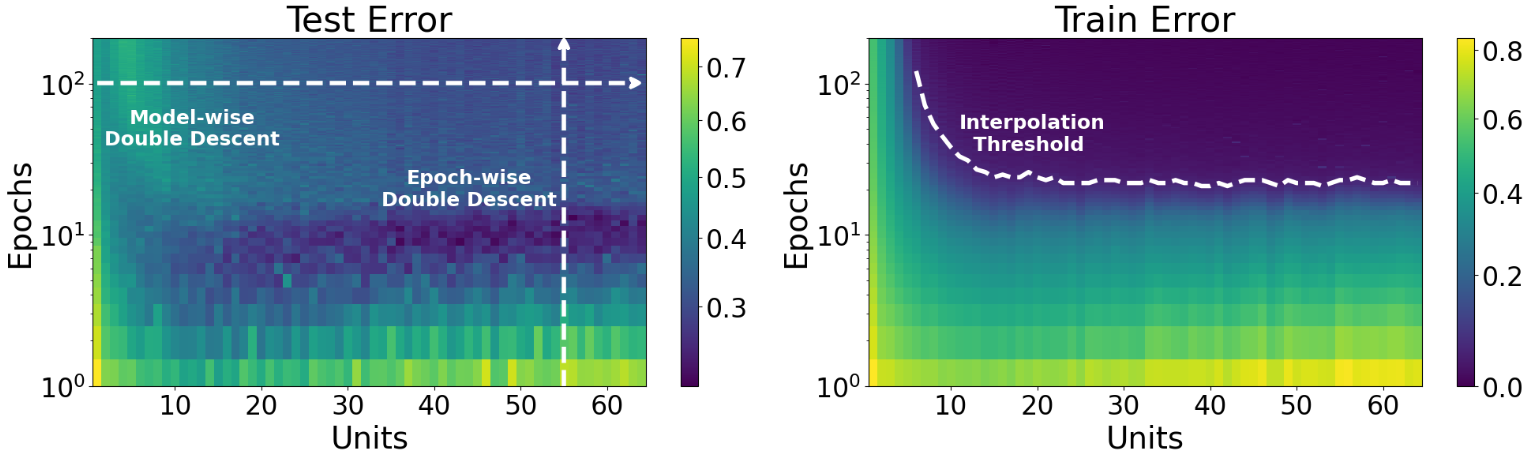
\includegraphics[width=0.95\textwidth]{img/experiments/model-epochPreActResNet18CIFAR10augmented.png}
    \caption[Doble descenso en función del tamaño del modelo y del número de épocas para la red ResNet$18$ y el conjunto CIFAR$10$.]{A la izquierda se muestra el error en prueba en función del tamaño del modelo y del número de épocas de entrenamiento. A la derecha, se representa el error de entrenamiento de los modelos correspondientes. Todas las arquitecturas consideradas son redes ResNet$18$ entrenadas en el conjunto CIFAR$10$ con aumento de datos\protect\footnotemark, $20\%$ de ruido añadido y durante $200$ épocas.}\label{fig:model-epochPreActResNet18CIFAR10}
\end{figure}
\footnotetext{A partir de este momento, siempre que se hace referencia a ``aumento de datos'' implicará el uso conjunto de \textit{RandomCrop($32$, $4$)} y \textit{RandomHorizontalFlip} como técnicas de transformación sobre el conjunto de entrenamiento.}

\begin{figure}[h]
    \centering
    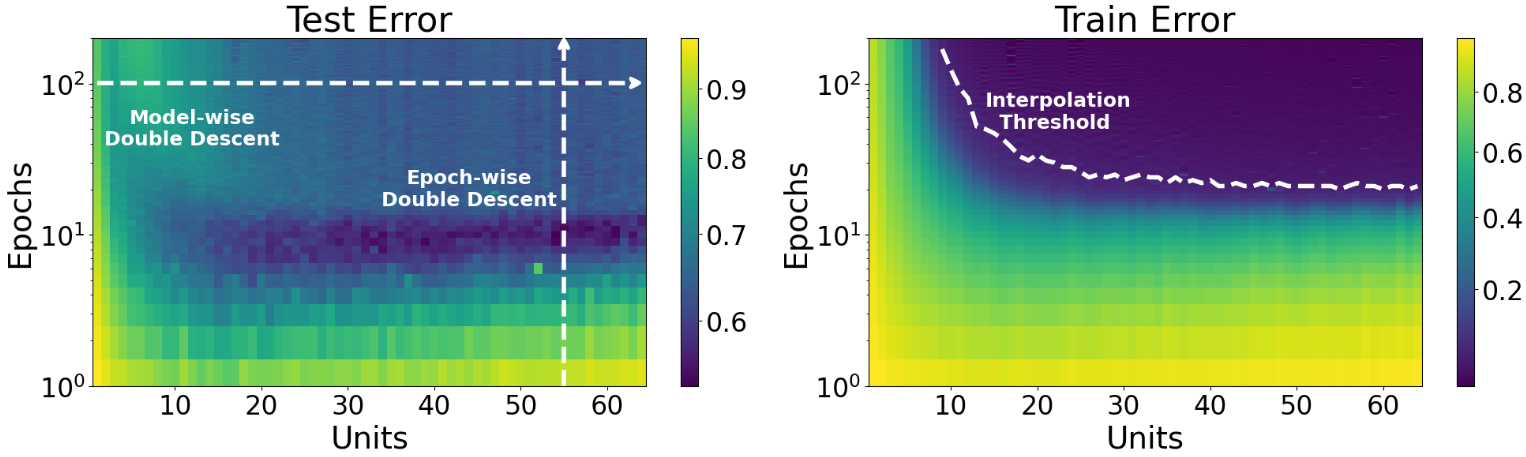
\includegraphics[width=0.95\textwidth]{img/experiments/model-epochPreActResNet18CIFAR100augmented.png}
    \caption[Doble descenso en función del tamaño del modelo y del número de épocas para la red ResNet$18$ y el conjunto CIFAR$100$.]{A la izquierda se muestra el error en prueba en función del tamaño del modelo y del número de épocas de entrenamiento. A la derecha, se representa el error de entrenamiento de los modelos correspondientes. Todas las arquitecturas consideradas son redes ResNet$18$ entrenadas en el conjunto CIFAR$100$ con aumento de datos, $20\%$ de ruido añadido y durante $200$ épocas.}\label{fig:model-epochPreActResNet18CIFAR100}
\end{figure}

\begin{figure}[h]
    \centering
    \begin{subfigure}[b]{0.48\textwidth}
        \centering
        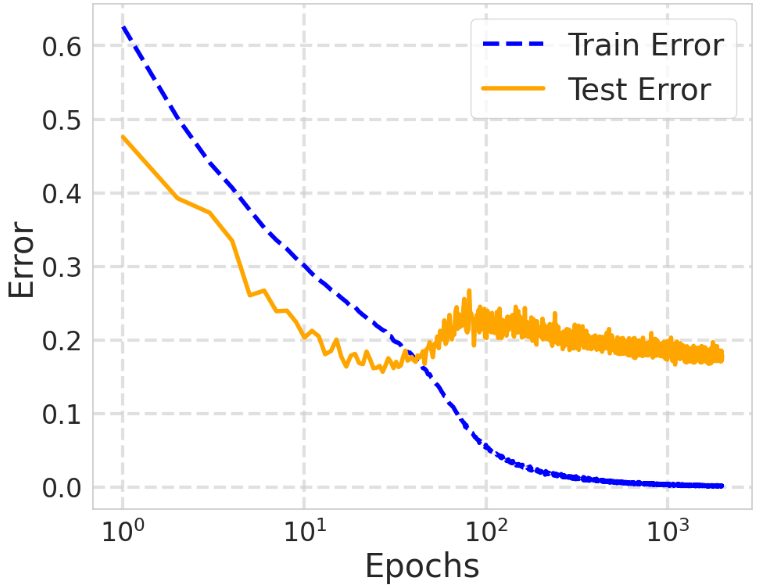
\includegraphics[width=\textwidth]{img/experiments/PreActResNet18(45).png}
        \caption{Doble descenso en función del número de épocas para la arquitectura ResNet$18$ con $k = 45$.}\label{fig:PreActResNet18(45)}
    \end{subfigure}
    \hfill
    \begin{subfigure}[b]{0.48\textwidth}
        \centering
        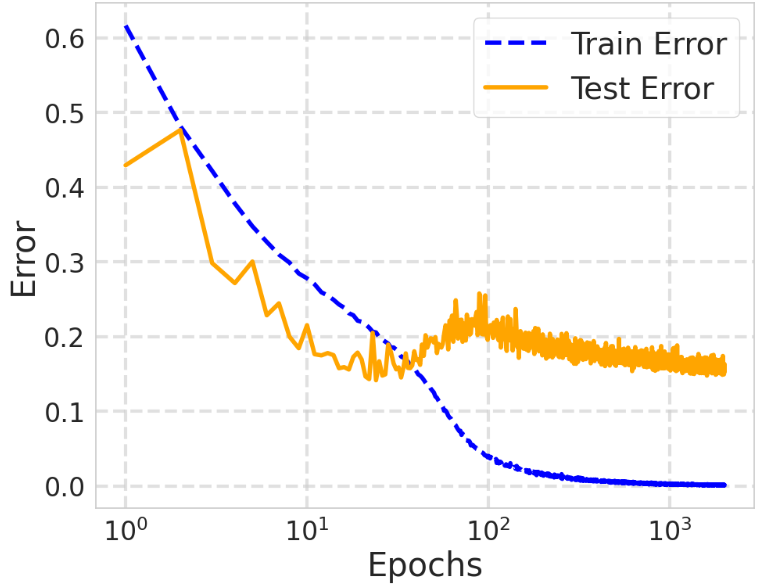
\includegraphics[width=\textwidth]{img/experiments/PreActResNet18(64).png}
        \caption{Doble descenso en función del número de épocas para la arquitectura ResNet$18$ con $k = 64$.}\label{fig:PreActResNet18(64)}
    \end{subfigure}
    \caption[Doble descenso en función del número de épocas para dos arquitecturas ResNet$18$ sobreparametrizadas y el conjunto CIFAR$10$.]{Doble descenso en función del número de épocas para dos arquitecturas ResNet$18$ sobreparametrizadas y el conjunto CIFAR$10$ con aumento de datos y $20\%$ de ruido añadido, entrenadas durante $2000$ épocas.}\label{fig:epoch-wisePreActResNet18over}
\end{figure}

\begin{table}[h!]
    \centering
    \begin{tabular}{|c|c|c|}
    \hline
    \textbf{Modelo}       & \textbf{Dataset} & \textbf{Entrenamiento} \\ 
    \hline
    PreActResNet$18$ ($1-64$) & MNIST ($10$\% label noise)        & $68$h $33$min \\ 
    PreActResNet$18$ ($1-64$) & CIFAR$10$  ($20$\% label noise)   & $86$h $17$min \\
    PreActResNet$18$ ($1-64$) & CIFAR$100$  ($20$\% label noise)   & $88$h $51$min \\
    PreActResNet$18$ ($45$) & CIFAR$10$  ($20$\% label noise)   & $21$h $26$min \\
    PreActResNet$18$ ($64$) & CIFAR$10$  ($20$\% label noise)   & $23$h \\
    \hline
    \end{tabular}
    \caption[Resumen de los experimentos para el doble descenso por complejidad del modelo y épocas para la red ResNet$18$ modificada.]{Resumen de los experimentos para el doble descenso por complejidad del modelo y épocas para la red ResNet$18$ modificada.}\label{tab:preactresnet_model-epochwise}
\end{table}

\subsubsection{Discusión}\label{subsubsec:discusion-model-epoch}

Para concluir, se exponen las conclusiones más significativas derivadas de este experimento:

\begin{itemize}
    \item Se han identificado numerosos casos favorables del fenómeno de doble descenso al utilizar diversas arquitecturas y conjuntos de datos. Además, se han observado casos desfavorables relacionados con la falta de capacidad de la arquitectura empleada para alcanzar su complejidad efectiva.
    \item El promedio entre épocas y parámetros en el que aparece el umbral de interpolación sigue una tendencia descendente hasta estabilizarse.
    \item Al entrenar modelos sobreparametrizados durante un gran número de épocas sin conexiones residuales, se observan saltos bruscos en los errores de entrenamiento y test, lo que está relacionado con la caoticidad del paisaje de la función de pérdida. No obstante, este paisaje resulta menos caótico cuando se emplean conexiones residuales.
\end{itemize}

\subsection{\textit{Width vs Depth double descent}}\label{subsec:width-depth}

En esta subsección se analiza cómo varía el \textit{Deep Double Descent} al emplear arquitecturas con la misma capacidad, pero con configuraciones diferentes. En particular, se comparan redes poco profundas y muy anchas con redes más profundas y poco anchas, dado que, según la teoría, ambas presentan comportamientos distintos ante un mismo problema~\cite{Nguyen2021}.

En la práctica, la literatura científica tiende a centrarse en redes anchas, cuya capacidad se incrementa aumentando el número de filtros en las capas convolucionales o el número de unidades ocultas en las capas densas. En contraste, existen pocos trabajos que exploren arquitecturas significativamente más profundas con la misma capacidad.

Para la realización de este experimento, se utilizan las arquitecturas $2$NN y $3$CNN como redes anchas y poco profundas. A partir de ellas, se incrementa la profundidad añadiendo capas densas a la $2$NN y capas convolucionales a la $3$CNN, y se reduce su anchura disminuyendo el número de neuronas y filtros por capa, manteniendo un número de parámetros similar. De esta forma, si consideramos que la red $2$NN cuenta con $2$ capas de profundidad ($2$ capas densas), la nueva red análoga profunda, DeepNN, cuenta con $8$ capas de profundidad. A su vez, la red $3$CNN cuenta con $3$ capas de profundidad ($3$ capas convolucionales, sin contar la capa densa de salida), y su red análoga profunda, DeepCNN, cuenta con $10$ capas de profundidad.

\begin{figure}[htbp]
    \centering
    \begin{subfigure}[b]{0.47\textwidth}
        \centering
        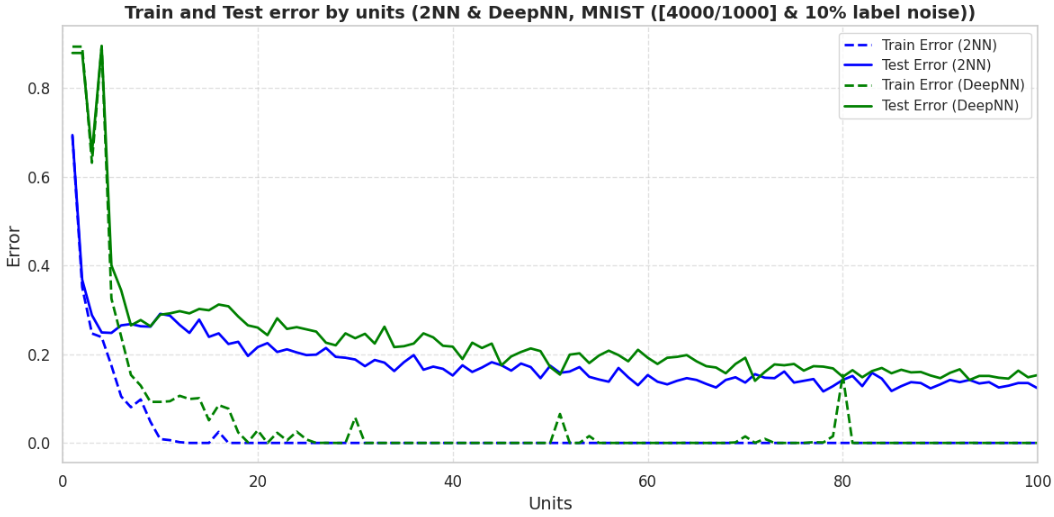
\includegraphics[width=\textwidth]{img/experiments/2nnvsdeepnn.png}
        \caption{Error de entrenamiento (línea discontinua) y test (línea continua) para dos arquitecturas (DeepNN y $2$NN) con similar número de parámetros pero distinta configuración sobre el subconjunto MNIST[$4000/1000$] con $10\%$ de ruido añadido.}\label{fig:2nnvsdeepnn}
    \end{subfigure}
    \hfill 
    \begin{subfigure}[b]{0.47\textwidth} 
        \centering
        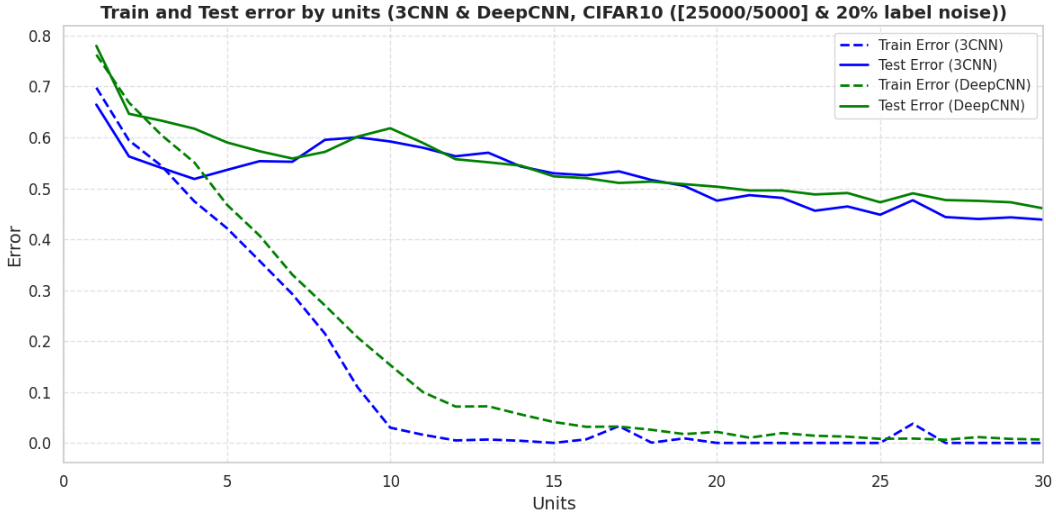
\includegraphics[width=\textwidth]{img/experiments/3cnnvsdeepcnn.png}
        \caption{Error de entrenamiento (línea discontinua) y test (línea continua) para dos arquitecturas (DeepCNN y $3$CNN) con similar número de parámetros pero distinta configuración sobre el subconjunto CIFAR$10$[$25000/5000$] con $20\%$ de ruido añadido y un \textit{batch size} de $128$.}\label{fig:3cnnvsdeepcnn}
    \end{subfigure}
    
    \caption[Comparativa del doble descenso entre arquitecturas anchas y profundas.]{Comparativa del doble descenso entre arquitecturas anchas y profundas.}\label{fig:width-depth}
\end{figure}

La Figura~\ref{fig:width-depth} muestra una comparación entre las arquitecturas análogas mencionadas en distintos conjuntos de datos. Se observa que el doble descenso se manifiesta de forma similar al aumentar la capacidad de una arquitectura, ya sea mediante mayor anchura o mayor profundidad. Asimismo, se observa que el umbral de interpolación se desplaza hacia la derecha al utilizar una red de mayor profundidad, ligado al hecho de que este tipo de arquitectura requiere más capacidad para alcanzar su complejidad efectiva (error de entrenamiento cercano a cero).

Como conclusión, aunque la experimentación sea limitada, estos resultados sugieren que el fenómeno podría ser, en cierta medida, robusto frente a la configuración utilizada, lo que indica que no es necesario crear arquitecturas tan profundas para observar su aparición, trabajando así con redes más compactas.

\subsubsection{Discusión}\label{subsubsec:discusion-width-depth}

Como resumen final, se presentan las conclusiones más relevantes derivadas de este experimento:

\begin{itemize}
    \item Al emplear redes profundas en lugar de redes anchas, se sigue manifestando el doble descenso, lo que sugiere que este es robusto frente a diferentes configuraciones dentro de una misma arquitectura.
    \item El umbral de interpolación se desplaza hacia la derecha al utilizar redes profundas, lo que está relacionado con la necesidad del modelo de una mayor capacidad para alcanzar su complejidad efectiva.
\end{itemize}

\section{Discusión comparativa global}\label{sec:conclusion-informatica}

A lo largo de esta sección se han presentado diversos experimentos destinados a analizar la aparición del doble descenso en distintas arquitecturas y conjuntos de datos. Asimismo, se han explorado casos en los que no se manifiesta.

El análisis comenzó con un ejemplo sencillo de regresión sobre datos sintéticos, sin emplear redes neuronales, utilizando la pseudoinversa para encontrar la solución. Este estudio puso de manifiesto la influencia de la base elegida, dado que al utilizar una base de polinomios de Legendre se observó el efecto, mientras que con las otras bases empleadas no se aprecia. También se evidenció cómo la presencia de ruido favorece su aparición y cómo las soluciones proporcionadas por la pseudoinversa favorecen aquellas con menor norma del vector de parámetros, tal como se explicó en la Sección~\ref{sec:svd-pseudoinversa}. Asimismo, se verificó que el modelo tiende a preferir soluciones más simples (suaves), en concordancia con los principios teóricos.

Posteriormente, se introdujo el concepto de \textit{noise-wise double descent}, destacando cómo el porcentaje de ruido incide tanto en la localización del máximo del error de generalización como en su magnitud. Se observó que, al aumentar el nivel de ruido, el máximo del error se desplaza hacia la derecha y se vuelve más pronunciado.

En el siguiente experimento, correspondiente al \textit{sample-wise double descent}, se identificó una región en la que incrementar la cantidad de datos de entrenamiento puede, de manera paradójica, empeorar el rendimiento. A su vez, se vuelve a observar un desplazamiento del máximo del error de generalización conforme se incrementa el número de ejemplos, y se estimó un valor promedio de la razón entre parámetros y ejemplos en el que dicho máximo suele situarse.

Finalmente, se abordaron los dos casos más representativos: el \textit{model-wise} y el \textit{epoch-wise double descent}, tratados de manera conjunta. En esta sección se incluyeron resultados obtenidos con múltiples arquitecturas y conjuntos de datos, lo que permitió estudiar en qué condiciones se reproduce el suceso. También se examinó si el comportamiento se presenta por igual en redes anchas y profundas.

Para concluir, se presenta la Tabla~\ref{tabla:resumen-experimentos} como resumen de los experimentos realizados, junto con una indicación sobre la presencia o ausencia del comportamiento en cada caso.

\begin{table}[h]
    \centering
    \begin{tabular}{ccccccc}
    \toprule
    & & & \multicolumn{3}{c}{Double - Descent} &  \\
    \cmidrule(lr){4-6}
    Conjunto de datos & Arquitectura & \% Ruido & Model & Epoch & Sample & Figura(s)  \\
    \midrule
    \multirow{2}{*}{Sintético} & Legendre base & $0$ & \cmark & -- & -- &~\ref{fig:legendre1DDD},~\ref{fig:legendrehyperbolicDD} \\
    & Polynomial base & $0$ & \xmark & -- & -- &~\ref{fig:OLS1DDD} \\
    \midrule
    \multirow{8}{*}{MNIST} & \multirow{3}{*}{$2$NN} & $0$ & \xmark & \xmark & -- &~\ref{fig:noise-wise-dd} \\
    &  & $10$ & \cmark & \cmark & \cmark &~\ref{fig:swdd},~\ref{fig:ratioparamsexamples} \\
    &  & [$20-40$] & \cmark & \cmark & -- &~\ref{fig:noise-wise-dd} \\
    \cmidrule(lr){2-7}
    & DeepNN & $10$ & \cmark & -- & -- &~\ref{fig:width-depth} \\
    \cmidrule(lr){2-7}
    & $3$CNN & $10$ & \cmark & \cmark & -- &~\ref{fig:model-epoch3CNNMNIST30k} \\
    \cmidrule(lr){2-7}
    & PreActResNet$18$ & $10$ & \cmark & \cmark & -- &~\ref{fig:model-epochPreActResNet18MNIST} \\
    \midrule
    \multirow{6}{*}{CIFAR$10$} & $2$NN & $20$ & \xmark & \xmark & -- &~\ref{fig:model-epoch2NNCIFAR10} \\
    \cmidrule(lr){2-7}
    & $3$CNN & $20$ & \cmark & \cmark & -- & ~\ref{fig:model-epoch3CNNCIFAR10} \\
    \cmidrule(lr){2-7}
    & DeepCNN & $20$ & \cmark & -- & -- & ~\ref{fig:width-depth} \\
    \cmidrule(lr){2-7}
    & PreActResNet$18$ & $20$ & \cmark & \cmark & -- & ~\ref{fig:model-epochPreActResNet18CIFAR10} \\
    \midrule
    \multirow{3}{*}{CIFAR$100$} & $3$CNN & $20$ & \cmark & \xmark & -- & ~\ref{fig:model-epoch3CNNCIFAR10025k} \\
    \cmidrule(lr){2-7}
    & PreActResNet$18$ & $20$ & \cmark & \xmark & -- & ~\ref{fig:model-epochPreActResNet18CIFAR100} \\
    \bottomrule
    \end{tabular}
    \caption[Resumen de los experimentos realizados sobre el doble descenso.]{Resumen de los experimentos realizados para los distintos tipos de doble descenso en función del conjunto de datos, la arquitectura y el porcentaje de ruido.}\label{tabla:resumen-experimentos}
\end{table}

\endinput